\documentclass[a4paper,11pt,twoside,openleft]{memoir}
\usepackage{lmodern}
\usepackage{amssymb,amsmath}
\usepackage{mathtools}
\usepackage{ifxetex,ifluatex}
\usepackage{fixltx2e} % provides \textsubscript
\ifnum 0\ifxetex 1\fi\ifluatex 1\fi=0 % if pdftex
  \usepackage[T1]{fontenc}
  \usepackage[utf8]{inputenc}
\else % if luatex or xelatex
  \ifxetex
    \usepackage{mathspec}
    \usepackage{xltxtra,xunicode}
  \else
    \usepackage{fontspec}
  \fi
  \defaultfontfeatures{Mapping=tex-text,Scale=MatchLowercase}
  \newcommand{\euro}{€}
\fi
% use upquote if available, for straight quotes in verbatim environments
\IfFileExists{upquote.sty}{\usepackage{upquote}}{}
% use microtype if available
\IfFileExists{microtype.sty}{\usepackage{microtype}}{}
\usepackage{longtable,booktabs}
\usepackage{graphicx}
\makeatletter
\def\maxwidth{\ifdim\Gin@nat@width>\linewidth\linewidth\else\Gin@nat@width\fi}
\def\maxheight{\ifdim\Gin@nat@height>\textheight\textheight\else\Gin@nat@height\fi}
\makeatother
% Scale images if necessary, so that they will not overflow the page
% margins by default, and it is still possible to overwrite the defaults
% using explicit options in \includegraphics[width, height, ...]{}
\setkeys{Gin}{width=\maxwidth,height=\maxheight,keepaspectratio}
\ifxetex
  \usepackage[setpagesize=false, % page size defined by xetex
              unicode=false, % unicode breaks when used with xetex
              xetex]{hyperref}
\else
  \usepackage[unicode=true]{hyperref}
\fi
\hypersetup{breaklinks=true,
            bookmarks=true,
            pdfauthor={Michele Pittoni},
            pdftitle={Advanced Topology Analysis in Three Wireless Community Networks},
            colorlinks=true,
            citecolor=blue,
            urlcolor=blue,
            linkcolor=black,
            pdfborder={0 0 0}}
\urlstyle{same}  % don't use monospace font for urls
\setlength{\parindent}{0pt}
\setlength{\parskip}{6pt plus 2pt minus 1pt}
\setlength{\emergencystretch}{3em}  % prevent overfull lines
\setcounter{secnumdepth}{0}
\usepackage[hypcap]{caption}
\usepackage{subcaption}
\usepackage[section]{placeins}
\usepackage{xspace}
\newcommand{\myName}{Michele Pittoni\xspace}
\newcommand{\myTitle}{Advanced Topology Analysis in Three Wireless Community Networks\xspace}
\newcommand{\myProf}{Prof. Renato Antonio Lo Cigno\xspace}
\newcommand{\figref}[1] {Figure~\ref{#1}}
\newcommand{\st}{\text{ st. }}
\newcommand{\etx}{\mathrm{ETX}}
\newcommand{\linkq}{\mathrm{LQ}}
\newcommand{\nlq}{\mathrm{NLQ}}
\newcommand{\mpr}{\mathrm{MPR}}
\newcommand{\mss}{\mathrm{MSS}}
\chapterstyle{section}

\title{Advanced Topology Analysis in Three Wireless Community Networks}
\author{Michele Pittoni}
\date{July 2014}

\begin{document}

\begin{titlingpage}
\pdfbookmark[1]{Titlepage}{Titlepage}
\changetext{}{}{}{((\paperwidth  - \textwidth) / 2) - \oddsidemargin - \hoffset - 1in}{}
\setulmargins{0.5cm}{*}{*}

\begin{center}
	\LARGE{UNIVERSIT\`A DEGLI STUDI DI TRENTO}
	
	\large
	Dipartimento di Ingengeria e Scienza dell'Informazione\\
	\begin{figure}[ht] 
    \center \includegraphics[height=30mm]{images/unitn_logo}
	\end{figure}
	\underline{UNIVERSITY OF TRENTO - Italy}\\
	\vspace*{10mm}
	Corso di Laurea in Informatica / Degree Course in Computer Science\\
	\rule{\linewidth}{1pt}
	\vspace*{10mm}
	Tesi finale / Final Thesis\\
	\vspace*{18mm}
	\huge{\bfseries \myTitle}
\end{center}
\vspace*{16mm}
\begin{flushleft}
	Relatore/Supervisor:\hspace{\stretch{2}}Laureando/Graduant:\\
	\myProf\hspace{\stretch{1}}\myName\\
	\vspace*{3mm}
  Correlatore/Co-supervisor:\\
  Dott. Leonardo Maccari\\
	\vspace*{3mm}
\end{flushleft}
\vspace*{15mm}
\normalsize
\begin{center}
	Anno Accademico 2013 - 2014
\end{center}

\vfill
\end{titlingpage}



\cleardoublepage

\tableofcontents

\chapter*{Introduction}\label{introduction}
\addcontentsline{toc}{chapter}{Introduction}

Wireless networking is changing the world. Not many years ago, the idea of
accessing the Internet with a mobile phone seemed crazy; nowadays, children
grow surrounded by technology and are used to expect this sort of information
ubiquity.

Cellular networks are usually not very performing with regard to speed and offer
a limited amount of traffic at prices that are considered quite high.
Meanwhile, they are not the only way to connect in mobility: municipalities
and commercial activities are building public Wi-Fi networks for their
citizens or customers, usually for free.

Laws that regulate wireless communications also evolved in recent years,
loosening the initial restrictions imposed on radio transmissions over
public areas.
Another step further was allowing network owners to open up their
networks to other people without bureaucratic hurdles and worries of being
prosecuted for traffic generated by other users.

Wireless Community Networks fit in this diversified scenario as an alternative
approach, which leverages existing technology to build networks in ways that 
were not foreseen.
They push the Wi-Fi standard to the limit of its efficiency, especially
in terms of range. They exist thanks to the volunteer actions of their members,
and the network grows with the community (most of the time, community is
first and the network follows).

They represent a challenge and an ideal place for experiments for a network
scientist, because they have features which are not found in any other network.
The hacker culture that permeates most community network project means that
information on the networks is readily available or easily obtained by just
asking.

The development of tailored network protocols for mesh networks, a category
of which Wireless Community Networks are part, is an active research field.
Traditional routing protocols have been shown to be poor suited to these
environments, for a variety of reasons.

Another topic which gathers much interest is the measuring of the performances
of these networks. Their decentralised nature makes difficult to analyse
the behaviour of traffic: just knowing its volume is a challenge, since in
theory every node should be monitored to acquire this information.

A reason which I've personally found exciting to examine Wireless Community
Networks is that they seem a credible approach toward a communication
infrastructure which is really a common good. An infrastructure owned by the
citizens and operated without central authorities seems a more than reasonable
approach, especially now that, according to the news, the era of mass Internet
surveillance has officially begun.

This thesis provides an introduction to the topic of Wireless Community Networks
(\hyperref[wireless-community-networks]{chapter 1})
and a survey of the mathematical methodologies used to analyse networks
(\hyperref[network-topology-and-graphs]{chapter 2}).
Chapter 2 also introduces two random network models which are subsequently
compared to real networks in their behaviour.
\hyperref[olsr-survey]{Chapter 3} then explains the most important 
features of OLSR, a popular routing protocol in Wireless Community Networks.

\hyperref[the-networks]{Chapter 4} describes the three networks which are
the object of the subsequent analysis, explaining their differences in terms
of history, community approach, internal organisation and, most importantly,
high level topological features.

\hyperref[robustness-analysis]{Chapter 5} and
\hyperref[message-propagation-analysis]{chapter 6} present the two metrics
analysed in the networks and in the random models.
The former analyses the robustness of the networks in different failure and
attack scenarios. There has been interest in literature to the behaviour
of many real world networks, which are quite robust to random failure but
collapse quickly in the case of a targeted attack. This analysis
extends this considerations also to the three Wireless Community Networks.

Chapter 6, on the other hand, examines the networks in a dynamic scenario
through a simulation of the exchange of routing information between nodes.
Wireless links are notoriously unreliable and the loss of packets negatively
impacts the diffusion of information on the topology.
Nodes which do not receive this information often enough may suffer from the
choice of suboptimal routes or even ignore the existence of other nodes.
This analysis shows the impact of link loss on routing information
in the three networks, simulation three routing protocols with different
signalling methodologies.

The simulations of chapters 5 and 6 have been conducted with the use of the
software package NetworkX\footnote{\url{http://networkx.github.io}}, a Python
library for graph manipulation that incorporates many algorithms and random
graph generators.

\chapter{Wireless Community Networks}\label{wireless-community-networks}

The term ``Wireless Community Network'' (WCN) is used in literature to
indicate various kinds of networks. The most common usage refers to
wireless mesh networks operated by a community of citizens, as opposed
to those controlled by a single entity (corporations or governments).
Other authors also use the term for the public hotspot networks run by
municipalities, or more generally for networks that provide wireless
connection to the public. In this document the term is used with the
first meaning, only for networks which are run -- not merely accessible
-- by the community.


\section{History}\label{history}

The appearance of the first Wireless Community Network can be dated to
the late 1990s-early 2000s, when the IEEE 802.11 protocol (Wi-Fi) was
first introduced.

They started as experiments by radio enthusiasts who
wanted to explore the potential of this new technology, pushing it to
the limit: Wi-Fi was designed as a protocol for local communication, but
it was shown that, with the right equipment, it can perform well also on
long distance links. The experimentation was made easier by the
unlicensed spectrum of frequencies in which Wi-Fi operates.

With Wi-Fi gaining popularity and wireless enabled devices becoming
mainstream, the cost of Wi-Fi equipment decreased and so did the barrier
to participate in WCNs. At the same time, wireless protocols evolved and
improved. For instance, 802.11a operates in the less crowded 5GHz band,
allowing more separation between the used frequencies and thus, less
interference.

In addition, a key factor to the diffusion on WCNs was the
scarce availability of broadband connections in certain areas. In such
cases, networks were not an experiment any more, but were used to provide
services where commercial initiatives were lacking.

Today, the WCN scenario has changed: in some places they are still used to
mitigate the digital divide, elsewhere they work as experimental
test beds or are more focused on the social/political aspect of being an
autonomous network owned and run by citizens. In the latter, the focus
is on the services provided inside the network rather than on Internet
access, which in some cases is not even available.

Some WCNs have grown to
the point of having an Autonomous System (AS) number assigned and being able to
peer with other networks at Internet eXchange Points (IXPs).

WCNs usually have a cultural background of Open Source enthusiasts and
hackers\footnote{as in ``curious'', not as in ``criminal''} in general.
Some of them are run by a formal associations, other by informal groups
of citizens, but in every case node owners know each other and there is
a sense of community. More experienced participants share their
technical knowledge (and their time), making it possible for new members
to enter the network with minimum effort.

Because of their spontaneous nature, it is difficult to
determine precisely the number of active WCNs as there is no central
registry to look at. However, there is a Wikipedia page\footnote{(``List
  of Wireless Community Networks by Region. Wikipedia, the Free
  Encyclopedia'' 2014)} which, albeit incomplete, lists 262 WCNs at the
time of writing. The dimensions of such networks vary from just a
handful of nodes to nearly 25,000 as in Guifi\footnote{\url{http://guifi.net}},
which is widely regarded as the world's largest WCN.

\section{Technology}\label{technology}

\begin{figure}[htbp]
\centering
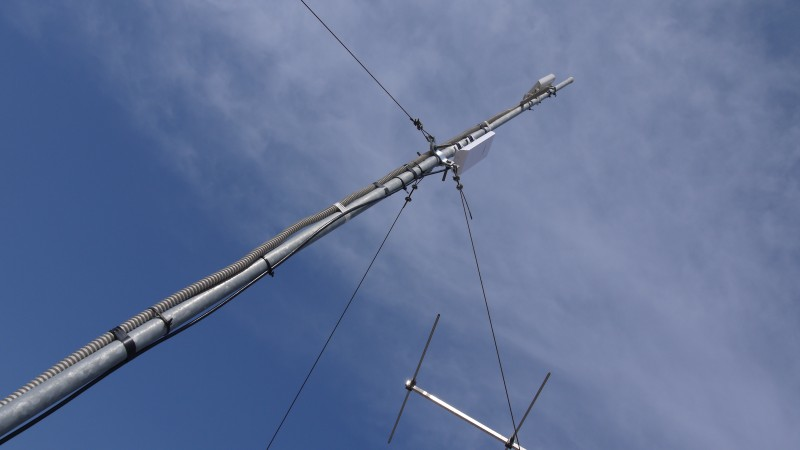
\includegraphics{images/ninux_node.png}
\caption{Antennas of a WCN node}
\end{figure}

WCNs were born together with the IEEE 802.11 protocol family and
continue to use it for various reasons, such as hardware availability
and low cost, unlicensed frequency spectrum operation and the constant
improvement of subsequent versions. Other solutions for the physical
layer are sometimes used -- for example proprietary protocols, maybe
operating in licensed frequencies, or even methods not based on
radio\footnote{Ronja, \url{http://ronja.twibright.com/}} -- but they are
an uncommon last resort when Wi-Fi can not work (due to interference or
other reasons).

A node of a WCN is a router connected with one or more radio interfaces.
There is not a standard for the construction of a node, but over time
every community has gathered some best practices and guidelines based on
experience and trial-and-error. The equipment used varies from consumer
Wi-Fi routers (such as the very popular Linksys WRT54GL) with home-made
antennas, to professional and more expensive equipment dedicated to
long-range Wi-Fi links. Smaller nodes, especially if they are close enough,
may use a single omnidirectional antenna to connect to
different nodes. Usually, however, directive antennas with a limited
beam width are used, to reduce interference leveraging different
channels, avoid receiving noise from all directions and achieve an
higher gain. Some nodes use both kinds of antennas, directive for
backbone links and omnidirectional to provides an hotspot access.

\begin{figure}[htbp]
\centering
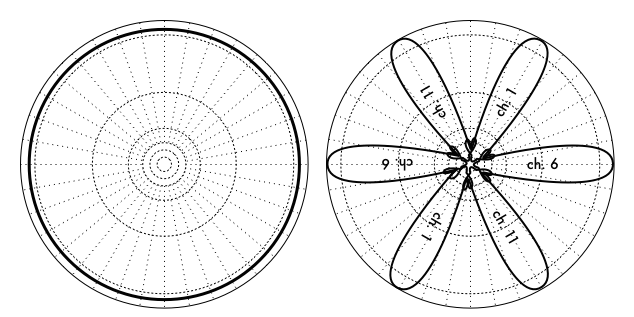
\includegraphics{./images/directional-antennas.png}
\caption{The difference between an omnidirectional and multiple
directive antennas.}
\end{figure}

\section{Mesh networks}\label{mesh-networks}
A mesh network is a type of network in which every node relays information
to other nodes. The advantage of using a mesh, rather than a
hierarchic structure, is that mesh networks can automatically configure
and adapt to changes, without the need for manual intervention.

Mesh networks also benefit from having redundant paths and being able to
adapt in case of failure of some links.

Mesh networks are usually wireless, since wired connections tend to be
more permanent and reliable, and when cables are laid usually configuring
the network is the smallest issue.

Wireless mesh networks have a large number of applications.
They are used in sensor networks, which employ small embedded devices that
communicate with each other to relay data to an observation point.
The ``One Laptop Per Child'' project, which developed laptops to give to
students in third-world countries, equipped them with mesh networking
capabilities to enable sharing without a network infrastructure.

Routing is one of the biggest challenges in wireless mesh networks. Due
to the nature of wireless links, traditional routing protocols
thought for wired networks perform poorly when applied to them. In
recent years, many new routing protocols have been proposed to address
this issue and today there is a competition with no clear winner. The
two most widely known routing protocols for wireless mesh and ad-hoc
networks are OLSR and B.A.T.M.A.N. The former, which is used in the three
WCNs analysed in this work, will be the subject of
\hyperref[olsr-survey]{chapter 3}.

\chapter{Network topology and graphs}\label{network-topology-and-graphs}

Some mathematical instruments are required to do any kind of description
or analysis of the topology of a network, or to explain the functioning
of a routing protocol.

One mathematical structure which is used to describe networks is the
\emph{graph}. A \emph{simple, undirected graph} is an ordered pair
$G = (V, E)$, where elements of $V$ are the \emph{nodes} (also called
\emph{vertices}) of the graph, while $E \subseteq \binom{V}{2}$ is the set of the
\emph{edges} of the graph. As a convention, in the rest of this thesis,
nodes will be denoted with $v_i$, $i \in \mathbb{N}$, without meaning any
particular ordering of the nodes. Also, for convenience, an edge
$\{v_i, v_j \}$ will be denoted $e_{ij}$.

An edge $e_{ij}$ is said to be \emph{incident} to the vertices $v_i$ and
$v_j$; equivalently, $v_i$ and $v_j$ are incident to $e_{ij}$. Two
vertices incident to the same edge are said \emph{adjacent}.

The graph is said simple since there are no loops (i.e.
$\{u,u\} \not\in E$) and each pair of vertices is connected by at most
one edge. The above mentioned graph is also said undirected. On the
other hand, a \emph{directed graph} is a pair $D = (V, A)$ where
$A = \{(u,v) \st u,v \in V,\, u \neq v\}$. The notation $(a,b)$ means
an ordered pair, in contrast to edges of an undirected graph
which are unordered. The elements of $A$ are
usually called \emph{arcs}.

For the purposes of describing networks, graphs are considered to be
\emph{finite}, so $V$ and $E$ are finite sets. Many well known finite
graph properties do not hold in the infinite case.

A \emph{weighted graph} is a graph in which every edge has an associated
label \emph{weight}, usually a real number. It is useful to define a
function $w: E \rightarrow \mathbb{R}$ which associates weights to
edges; in the case of unweighted graphs, it can be assumed
$w: e \mapsto 1\, \forall e \in E$.

To model networks as graphs, each node of the network is represented by
a node in the graph and a link between two nodes is represented by an
edge between those nodes. If there are unidirectional link, a directed
graph is used. In the routing protocol used by the networks analysed here,
only bidirectional links are used, and the quality of a link is measured
on the round-trip, so it is symmetrical. Given so, from now on ``graph''
will be used for simple, undirected graphs.

\section{Terminology}\label{terminology}

This section introduces the terminology that will be used throughout
the thesis when referring to graph properties.

\subsection{Order and size}\label{order-and-size}

The \emph{order} of a graph is the number of its nodes, $|V|$. The
\emph{size} of a graph is the number of its edges, $|E|$.

\subsection{Degree}\label{degree}

The \emph{degree} $k_v$ of a vertex $v$ is the number of edges incident
to that vertex. A vertex of degree 0 is an \emph{isolated vertex}. A
vertex of degree 1 is a \emph{leaf}.

The \emph{total degree} of a graph is $\sum_{v \in V} k_v$.

The \emph{degree sequence} of a graph is the list of degrees in
non-increasing order.

The \emph{degree distribution} of a graph is a function
$p_k: \mathbb{N} \rightarrow [0, 1]$ such that

\begin{equation*}
p_k(n) = \frac{\left\vert{ \{v \in V \st k_v = n\} }\right\vert}{|V|}
\end{equation*}

The degree distribution is a discrete probability distribution since
$\sum_{k} p_k = 1$.

\subsection{Subgraphs}\label{subgraphs}

The set $E$ of the edges of graph $G$ can also be seen as a relationship
between the vertices of the graph. This means that given a subset of the
vertices, $V' \subseteq V$, the restriction $E\restriction_{V'}$ can be
defined. As a set, $E\restriction_{V'} \coloneqq
\{\{v_i, v_j\} \in E \st v_i,v_j \in V'\}$

A \emph{subgraph} $G' = (V', E')$ of $G$ is a graph such that
$V' \subseteq V$ and $E' \subseteq E\restriction_{V'}$.

\subsection{Walks, paths}\label{walks-paths}

A \emph{walk} is a sequence of vertices
$P = (v_0, v_1, \ldots, v_n) \in V \times V \times \ldots \times V$ such
that $\{v_i, v_{i+1}\} \in E,\, 0 \leq i < n$. A walk is \emph{closed} if
$v_0 = v_n$, \emph{open} otherwise. The \emph{length} of the walk is
$n$. The \emph{weight} of the walk is
$w_P = \sum_{i=0}^{n-1} w(\{v_i, v_{i+1}\})$. In unweighted graphs, $w_P = n$.

A \emph{path} is a walk with no repeated vertices. A \emph{cycle} is a
closed walk with no repeated vertices, except obviously the starting one
which is repeated once at the end.

Given a graph with no negative-weight cycles, a \emph{geodesic path},
also called \emph{shortest path}, between $v_0$ and $v_n$ is a walk
$P = (v_0, v_1, \ldots, v_n)$ such that
$\nexists P' = (u_0, u_1, \ldots, u_m)$ with
$u_0 = v_0,\, u_m = v_n \st w_{P'} < w_P$.\\
In a graph with negative-weight cycles, the
geodesic path is not defined, since it is possible to have walks with
$w_P = -\infty$.\\
The length of a geodesic path (which is the length of
all of them) from $u$ to $v$ is called \emph{geodesic distance} of $u$
and $v$, indicated with $d_{uv}$

\subsection{Neighbours}\label{neighbours}

Each vertex adjacent to $v$ is also called a \emph{neighbour} of $v$.
The set of the neighbours of $v$ is called \emph{neighbourhood} of $v$.

The concept of neighbourhood may be extended to vertices at any
distance. For example, the \emph{2-hop neighbourhood} of $v$ is the set
of vertices $u$ such that there is a walk from $v$ to $u$ with length 2.
Similarly, the \emph{strict 2-hop neighbourhood} of $v$ is the set of
vertices which are in the 2-hop neighbourhood, excluding $v$ itself and
its direct neighbours.

\subsection{Connectivity}\label{connectivity}

A graph is called \emph{connected} if, for each pair $\{u,v\}$ of nodes,
there is a path between $u$ and $v$.

A \emph{connected component} of $G$ is a maximally connected subgraph of
$G$.

\subsection{Centrality}\label{centrality}

In network science there is substantial interest in the concept of the
centrality of a vertex (or an edge) in a graph. The idea behind this
metric is to determine the most ``important'' components of a network.
The meaning of ``important'' varies depending on the context: in social
networks importance is usually defined by the influence of a node,
measured by the size of it neighbourhood. In communication networks, the
most important nodes are those who participates to most communications,
either by forming circuits or by relaying packets. These are just two
examples of different notions of importance that require different ways
to be measured. The following paragraphs present the centrality metrics
relevant to this thesis.

\subsubsection{Degree centrality ($C_D$)}\label{degree-centrality}

The degree of a vertex is the simplest possible measure of centrality
and it is the only one that is only based on local properties. This is
an advantage from the computational point of view, but it also implies
that degree centrality is the least significant centrality metric.
Nonetheless, depending on the graph, it can approximate quite well the
behaviour of other metrics.

\begin{equation}
C_D(v) = k_v
\end{equation}

\subsubsection{Betweenness centrality ($C_B$)}\label{betweenness-centrality}

Betweenness centrality of vertex $v$ is defined as the fraction of
shortest paths between any two vertices that pass through $v$. Formally,
define $\sigma(s,t)$ the number of shortest paths from $s$ to $t$ and
$\sigma(s,t|v)$ the number of those paths that pass through $v$. If
$s = t,\, \sigma(s,t) = 1$. There is not a consensus in literature if a
path ``passes through'' its endpoint; in this case, it is assumed not:
$\sigma(s,t|s) = \sigma(s,t|t) = 0$. The betweenness centrality is

\begin{equation}
C_B(v) = \sum_{s,t \in V} \frac{\sigma(s,t|v)}{\sigma(s,t)} %_
\end{equation}

betweenness centrality is especially useful in the study of communication
networks because information usually travels through the shortest path,
so $C_B$ helps estimating how much traffic a node will see, in a way
other centrality measures do not consider. For example, in the classic
Barbell graph -- two complete graphs connected by a path -- vertices on
the path have a very small degree but since every path between the two
complete graphs passes through them they have high betweenness. This
reflects the big control they have over the communications between other
nodes.

\subsubsection{Edge betweenness centrality ($C_E$)}
\label{edge-betweenness-centrality}

The concept of betweenness centrality can also be easily extended to
edges, with a similar notation.

\begin{equation}
C_{E}(e) = \sum_{s,t \in V} \frac{\sigma(s,t|e)}{\sigma(s,t)}
\end{equation}

\subsubsection{Closeness centrality ($C_C$)}\label{closeness-centrality}

Closeness centrality is also based on shortest paths, but has a
different approach and a different meaning. It is based on the mean
distance between $v$ and the other vertices. If $d_{vu}$ is the geodesic
distance between $v$ and $u$, the \emph{mean geodesic distance} of $v$,
averaged over all vertices is

\begin{equation}
\mathcal{L}_v = \frac{1}{n} \sum_u d_{vu}  %_
\end{equation}

Since usually centrality metrics have high values for more central
nodes, closeness centrality is usually defined as the inverse of the
mean distance $\mathcal{L}_v$.

\begin{equation}
C_C(v) = \frac{1}{\mathcal{L}_v} = \frac{n}{\sum_u d_{vu}}  %_
\end{equation}

Closeness centrality, despite being often used in network studies, has
shortcomings. For example, the above definition is only valid if
the graph is connected, since $d_{vu}$ is defined to be infinite if
there is no path from $v$ to $u$. In graphs with more than one connected
components, $C_C$ would then be zero for every vertex. The usual
solution is to compute the closeness centrality for each connected
component separately: this works, but since distances are usually
smaller in small components, vertices in those components tend to have
higher closeness centrality, which may be undesirable.

Another issue with closeness centrality is that its values are often
cramped in a small range from lowest to highest. In most networks
distances tend to be small, typically increasing with the logarithm of
the size $n$ of the graph. So, the lower and upper bound for
$\mathcal{L}_v$ are, respectively, $1$ and $\log n$. Similarly, the
range for $C_C$ is limited.

\section{Random graph models}\label{random-graph-models}

A random graph is a graph generated by a random process. The reason for
using random graph models in network analysis is that they can produce
graphs with known degree distributions, which can be used to prove
mathematically or otherwise analyse empirically their structural and
dynamical properties.

\subsection{Erd\H{o}s-Rényi random
graph}\label{erdos-renyi-random-graph}

The random graph model originally proposed by Erd\H{o}s and Rényi is
also called $G(n,M)$ model, since it consists in the uniform random
selection of a graph from the set of all graphs with $n$ nodes and $M$
edges.

The model used here is a variation first introduced by (Gilbert 1959),
called the $G(n,p)$ model. The algorithm starts form a graph with $n$
nodes and no edges. Then, for each unordered pair of nodes
$\{i,j\} . i \neq j$, the edge $ij$ is added with probability $p$.

The $G(n,p)$ models has some interesting properties which are not
obvious at a first look. For example, the number of edges is not known
as in the $G(n,M)$ models, but the expected number of edges can be
determined to be $\binom{n}{2}p$. Another important aspect is
connectedness: with a large enough $n$,
for $p > \frac{(1+\epsilon) \ln n}{n}$ the graph will
almost surely be connected, while for $p < \frac{(1-\epsilon) \ln n}{n}$
it will almost surely have isolated vertices.

Finally, the degree distribution has the form

\begin{equation}
p_k = \binom{n-1}{k} p^k (1-p)^{n-1-k}
\end{equation}

\subsection{Barabási-Albert graph}\label{barabuxe1si-albert-graph}

A scale free network is a network whose degree distribution follows a
power law of the form

\begin{equation}
p_k = Ck^{-\alpha}
\end{equation}

A method for generating graphs with a power law degree distribution,
using a preferential attachment mechanism, was devised by A. L. Barabási
and R. Albert in (Barabási and Albert 1999). This is the method
implemented by NetworkX. Given a target number $n$ of nodes and a
parameter $m$ which controls the density of the network, the algorithm
starts from a graph with $m$ nodes and no edges. Then other nodes are
added and from each new node $m$ edges are created. The probability of an
existing node to be chosen as the destination of a new link is proportional
to its degree -- this is the meaning of preferential attachment.
The procedure continuesuntil there are $n$ nodes in the graph,
meaning the final graph will contain $(n-m) m$ edges.

\chapter{Survey of the OLSR protocol}\label{olsr-survey}

Optimized Link State Routing (OLSR) is a proactive routing protocol
standardized by the IETF in RFC 3626\footnote{Clausen and Jacquet (2003)}
and designed to have a better performance on wireless mesh and ad-hoc
networks than traditional protocols for wired networks.

In link state routing protocols, each node is supposed to know the
entire topology of the network in order to calculate the routes. This
means that each time the topology changes, the new information must be
propagated to every node. This is traditionally done by flooding
link-state advertisement packet through the network.

In the case of traditional networks with wired links, this method is
acceptable since the topology seldom changes. In WCN (and wireless
networks in general), however, links change their cost quite often and
may also disappear temporarily. Flooding in this situation imposes a big
effort on the network and may degrade the performance consistently.

OLSR addresses this concern with an optimized flooding mechanism which
significantly reduces the overhead by using only selected nodes, called
multipoint relays (MPRs), to broadcast link-state advertisements. The
next sections outline the details of this mechanism and of OLSR in
general.

\begin{figure}[htbp]
\centering
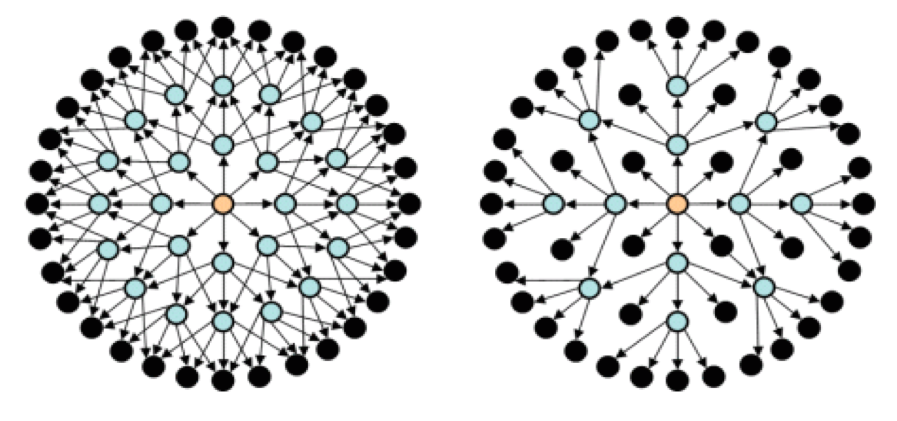
\includegraphics{images/mpr.png}
\caption{Flooding vs. MPR forwarding}
\end{figure}

\section{Generic packet format}\label{generic-packet-format}

OLSR uses different types of messages in its specification. In order to
take advantage of the maximal frame size provided by the network, one or
more messages are encapsulated in a packet which has the same format for
all types of messages. This facilitates the extensibility of the
protocol and allows the transmission of different kinds of information
in a single packet.

Each message is flooded through the network with a TTL. The transmission
to neighbours is just a special case of flooding with TTL=1. Duplication is
eliminated locally, since each node records the originator address and
sequence number of all the messages it processes.

\begin{figure}
\begin{verbatim}
 0                   1                   2                   3
 0 1 2 3 4 5 6 7 8 9 0 1 2 3 4 5 6 7 8 9 0 1 2 3 4 5 6 7 8 9 0 1
+-+-+-+-+-+-+-+-+-+-+-+-+-+-+-+-+-+-+-+-+-+-+-+-+-+-+-+-+-+-+-+-+
|        Packet Length          |    Packet Sequence Number     |
+-+-+-+-+-+-+-+-+-+-+-+-+-+-+-+-+-+-+-+-+-+-+-+-+-+-+-+-+-+-+-+-+
|  Message Type |     Vtime     |         Message Size          | 
+-+-+-+-+-+-+-+-+-+-+-+-+-+-+-+-+-+-+-+-+-+-+-+-+-+-+-+-+-+-+-+-+
|                      Originator Address                       |
+-+-+-+-+-+-+-+-+-+-+-+-+-+-+-+-+-+-+-+-+-+-+-+-+-+-+-+-+-+-+-+-+
|  Time To Live |   Hop Count   |    Message Sequence Number    |
+-+-+-+-+-+-+-+-+-+-+-+-+-+-+-+-+-+-+-+-+-+-+-+-+-+-+-+-+-+-+-+-+
|                                                               |
:                            MESSAGE                            :
|                                                               |
+-+-+-+-+-+-+-+-+-+-+-+-+-+-+-+-+-+-+-+-+-+-+-+-+-+-+-+-+-+-+-+-+
|  Message Type |     Vtime     |         Message Size          | 
+-+-+-+-+-+-+-+-+-+-+-+-+-+-+-+-+-+-+-+-+-+-+-+-+-+-+-+-+-+-+-+-+
|                      Originator Address                       |
+-+-+-+-+-+-+-+-+-+-+-+-+-+-+-+-+-+-+-+-+-+-+-+-+-+-+-+-+-+-+-+-+
|  Time To Live |   Hop Count   |    Message Sequence Number    |
+-+-+-+-+-+-+-+-+-+-+-+-+-+-+-+-+-+-+-+-+-+-+-+-+-+-+-+-+-+-+-+-+
|                                                               |
:                            MESSAGE                            :
|                                                               |
+-+-+-+-+-+-+-+-+-+-+-+-+-+-+-+-+-+-+-+-+-+-+-+-+-+-+-+-+-+-+-+-+
:                                                               :
               (etc.)
\end{verbatim}
\caption{Fields of a generic OLSR packet}
\end{figure}

\section{Link sensing and neighbour
discovery}\label{link-sensing-and-neighbour-discovery}

Link sensing and neighbour discovery are achieved in OLSR with the
use of \texttt{HELLO}
messages, which are transmitted by each node to its neighbours and
contain the addresses of the neighbours it knows. Of course, the first
\texttt{HELLO} messages are empty and only serve the purpose of link
sensing. After each node populates its neighbour set, it includes this
information in its \texttt{HELLO} messages, along with some information
on the links and the neighbours (e.g. if the links are verified to be
symmetric). This allows all nodes to gather the necessary knowledge of
their 2-hop neighbourhood. Only bidirectional links are considered by
OLSR as valid.

\texttt{HELLO} messages are generated and transmitted at a regular
interval (\texttt{HELLO\_INTERVAL}). Lost links are also advertised for
some time (with a link type of \texttt{LOST\_LINK}).

\section{MPR selection and
signalling}\label{mpr-selection-and-signalling}

Using the information from the \texttt{HELLO} messages, each node can
select a set of its neighbours such that every node in its 2-hop
neighbourhood is at 1 hop from the set. Formally, call $N_1(v)$ the
neighbourhood, $N_2(v)$ the strict 2-hop neighbourhood, select
$\mpr(v) \subseteq N_1(v)$ such that

\begin{equation*}
%*
\forall u \in N_2(v) \, \exists s \in \mpr(v) \text{ st. } u \in N_1(s)
\end{equation*}

This requirement essentially means that each node in the strict 2-hop
neighbourhood can be reached through a MPR. Once a node has selected its
MPRs, it needs to signal its choice to the neighbours.
\texttt{HELLO} messages are used also for this purpose:
the selected MPRs are advertised with a neighbour type of \texttt{MPR\_NEIGH}.

As a notational convention, $v \to u \Leftrightarrow u \in \mpr(v)$.

\section{Message forwarding}\label{message-forwarding}

Observing the \texttt{HELLO} messages it receives, node $v$ populates
and maintains an \texttt{MPR Selector Set}. This is the set

\begin{equation*}
  \mss(v) \coloneqq \{ u \in V \st u \to v \}
\end{equation*}

Node $v$ then need to retransmit only the messages it receives by nodes
in $\mss(v)$.

When $v$ receives a message (except for \texttt{HELLO} messages,
which are never forwarded), it checks if the time-to-live has reached
zero or if the message was already processed (by examining the duplicate
set). If the message passes this preliminary checks, it is forwarded
only if it was received from a selector.

The primary goal of using MPRs is reducing the number of duplicate message
retransmissions while ensuring that each node receives the required
information. The selection of MPR nodes influences the capacity of reaching
this goal. The OLSR specification suggests that the size of the MPR set
should be minimized. However, it leaves freedom to the implementer or
the network administrator to override the default heuristic in order to
achieve, for instance, more redundancy.

\section{Topology control}\label{topology-control}

The link-state information is propagated throughout the network with
\texttt{Topology Control} messages (\texttt{TC}). This messages are
generated only by the MPRs and propagated following the above described
rules. Each \texttt{TC} message contains the identification of the node who
generated the message and a list of the addresses of its
neighbours, but not all neighbours are necessarily included.

The OLSR specification requires that the nodes in the
\texttt{MPR Selector Set} of a node be in the \texttt{TC} messages it
generates. To add redundancy, each node can advertise, in addition, the
neighbours selected by it as MPRs, or even all of its neighbours. The
added redundancy comes at the cost of longer \texttt{TC} messages, which
may be more susceptible to congestion.

The links between an MPR and the neighbours that it does not advertise
in \texttt{TC} messages effectively disappear from the topology which is
known to other nodes. Thus, nodes in OLSR have only a partial knowledge
of the network and can calculate routes with this incomplete
information.

\section{Link quality}\label{link-quality}

OLSR implements a mechanism to avoid using ``bad'' links (links which
are usually too weak but may let \texttt{HELLO} messages pass from time
to time). Since \texttt{HELLO} messages are transmitted at a regular
interval, each node knows how many of them to expect from each neighbour
over a period of time. Comparing this with the number of received
messages it computes a measure of the Link Quality (LQ). This metric was
originally only used to decide if a link was reliable enough to use. New
versions of OLSR have put more importance on link quality.

It is common in WCNs to use the ETX metric to express link quality. ETX
stands for Expected Transmission Count and was proposed in De Couto
(2004). It indicates the expected number of transmissions (including
retransmissions) required to successfully deliver a packet.

In OLSR, ETX is derived directly from LQ. \texttt{HELLO} messages
contain the calculated values, so each node has for every link two
measures: its own (LQ) and its neighbour's (NLQ). Since each unicast packet
transmission requires an acknowledgement, the estimated probability of
success is $\linkq \cdot \nlq$. ETX is calculated as

\begin{equation}
\etx = \frac{1}{\linkq \cdot \nlq}
\end{equation}

The measure of ETX in OLSR is surely an approximation because it does not
describe the behaviour of real data packets. Only relatively small broadcast
packets are taken into account and this may introduce a bias since bigger
packets have more probability to be involved in collisions.
In addition, no regard is given to the possibility of getting a link quality
measure from the radio layer.

\section{Use of LQ in MPR selection}\label{use-of-lq-in-mpr-selection}

The heuristic proposed in the RFC to compute the MPR set of a node gives
no importance to link quality. This means that a node could choose as an
MPR a neighbour with a weak connection. Since MPRs advertise the route
to their selectors, this weak link may end up being used in place of a
better one, because the latter is not shared with an MPR.

To address this issue, it has been proposed to use an algorithm for
selecting MPRs that accounts for link quality. Unfortunately, the
rapidly changing nature of link quality causes instability in the MPR
set. This in turn causes MPRs to generate \texttt{TC} messages more
often, leading to an increase in signalling, the exact opposite of the
reason why MPR were introduced in the first place.

To avoid this effect, but still ensure that good links are not discarded
for weak ones, the implementation of OLSR used by the analysed WCNs
forces each node to be an MPR. Every node has thereby the complete
knowledge of the network topology.

\chapter{The networks}\label{the-networks}

The three WCNs which are analysed in the theses are Ninux (in Italy),
FunkFeuer Wien and FunkFeuer Graz (in Austria). The study considers 50
snapshots of the networks taken in January 2014.

\begin{center}
  \begin{tabular}{@{}rccc@{}}
  \toprule\addlinespace
  & Ninux & FFWien & FFGraz
  \\\addlinespace
  \midrule
  date & 20/01/14 & 13/01/14 & 13/01/14
  \\\addlinespace
  snapshot interval & 5 min & 5 min & 10 min
  \\\addlinespace
  timespan & 4h 10min & 4h 10min & 8h 20min
  \\\addlinespace
  \bottomrule
  \addlinespace
  \end{tabular}
  \captionof{table}{Details of the data collection}
\end{center}

The snapshots were obtained by the interpolation of the OLSR topology
exported directly by the routing daemons on the nodes (since each node
has the complete knowledge of the topology) and information published
(or otherwise provided) by the communities.

Some supernodes with several antennas make each of them run OLSR as an
independent node, connecting them to a switch. These cases have been
considered a single node for the purpose of this analysis, since they
represent devices in a single location, run by a single person and
connected to a single power source. Moreover, this type of configuration
is being replaced by a more efficient one, which uses a single router
running OLSR. The separate devices are then configured as simple 802.11
Access Points/clients and connected to the router using separate VLANs.

\section{Ninux}\label{ninux}


\includegraphics{images/ninux_logo.png} Ninux\footnote{\url{http://wiki.ninux.org/}}
is the largest Italian WCN. It was started in 2001 in Rome and now
consists of about 250 active nodes, located in different ``Ninux
islands'' all over Italy. The name ``Ninux'' originally was a tribute to
the project founder, Nino, but now the project members usually take it
with the meaning ``Neighbourhood Internet, Network Under eXperiment''.

Ninux is managed in an informal way: every member is the owner and
responsible of its node (or nodes), but there is no formal association.
This is a deliberate choice of the Ninux community, motivated by the
excessive bureaucratic effort it would require. Moreover, all
associations must have a president responsible for the activities of the
association itself, and Ninux members prefer the responsibility to be
decentralised (as the network is).

The different islands use a variety of protocols and have different
topologies:

\begin{itemize}
\itemsep1pt\parskip0pt\parsep0pt
\item
  in Pisa, Sicily and Friuli there are three mesh networks, with routing
  based on B.A.T.M.A.N.
\item
  in Rome, the biggest Ninux island uses a backbone with point-to-point
  links combined with some mesh areas, employing OLSR for all the
  routing
\item
  in recent years other networks have been created in Florence, Viterbo,
  Catanzaro, Cosenza and Reggio Calabria, all based on OLSR
\end{itemize}

The islands are connected together by tunnels using a variety of
protocols.

Ninux is an Autonomous System (AS\# 197835)\footnote{\url{https://apps.db.ripe.net/search/query.html?searchtext=AS197835\&object_type=aut-num\#resultsAnchor}}
and it is a member of the NaMeX\footnote{\url{http://www.namex.it/en/who/members}}
Internet Exchange Point.

In this work, the biggest Ninux island has been analysed (since it is
the biggest OLSR routing domain), which is Rome's network. It consists
of 132 nodes connected by 154 links (average degree of 2.333).

\begin{figure}[htbp]
\centering
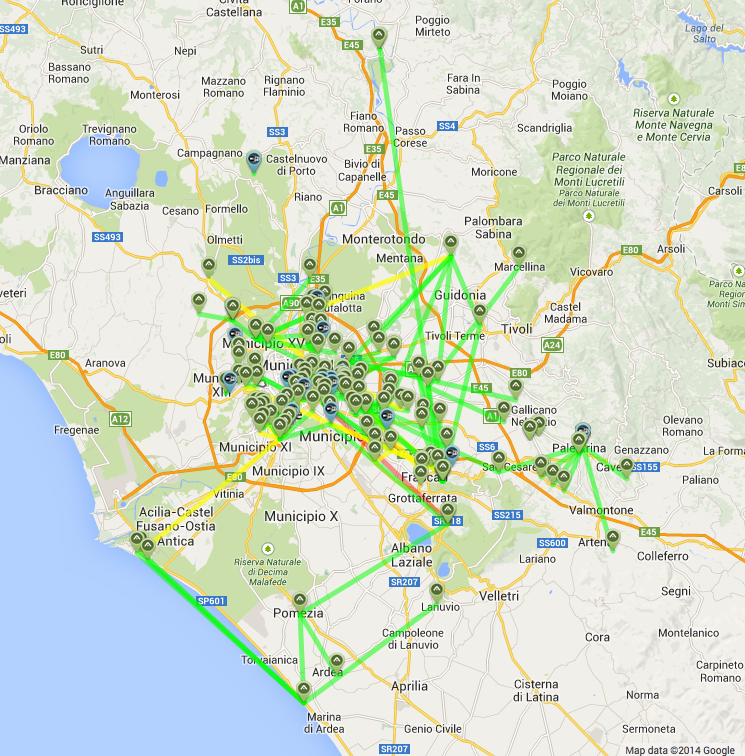
\includegraphics{images/ninux_map.png}
\caption{Map of the Rome Ninux island}
\end{figure}

\section{FunkFeuer: Wien}\label{funkfeuer-wien}

FunkFeuer\footnote{\url{http://www.funkfeuer.at/}} is a project that
comprises networks in different places of Austria (Vienna, Graz, parts of
Weinviertel and Bad Ischl). The literal meaning of ``funkfeuer'' in
German is ``radio beacon''. FunkFeuer is also a registered association
in Austria, differently from Ninux.

The origins of FunkFeuer are in the experiments of an Austrian ISP based
in Vienna, Silver Server, which, during the 1990s, explored the
commercial viability of wireless radio data links. After a test phase,
Silver Server ultimately decided that the technology was not ready to be
used commercially; however, the infrastructure was already in place and
it was handed off to two associations, Team Teichenberg and Public Voice
Lab. With direction from Franz Xaver and Roland Jankowski, they further
expanded the network, bringing the node count to 15, but failed to
create easy end-user access.

The network was ultimately decentralised, giving the opportunity to the
citizens to buy the hardware of the nodes. The advent of cheap GNU/Linux
based embedded Wi-Fi products promoted the growth of the network and an
association was founded to have a more structured organisation and
address the issues of decentralisation. The existence of a formal
association also enables to request sponsoring from local
administrations.

FunkFeuer Wien (FFWien)\footnote{\url{http://www.funkfeuer.at/Vienna.206.0.html?\&L=1}}
is the biggest of FunkFeuer networks, covering 1/3 of the city. The
active node in the analysed snapshots were 237, with 433 links (an
average degree of 3.654).

\section{FunkFeuer: Graz}\label{funkfeuer-graz}

FunkFeuer Graz (FFGraz)\footnote{\url{http://graz.funkfeuer.at/}} is the
``smaller sister'' of the FFWien network, situated in the homonymous
city. It was founded after FFWien by Othmar Gsenger, Erwin Nindl and
Roland Jankowski and has its own association to apply for local
sponsoring. It consists of 144 nodes and 199 edges, with an average
degree of 2.764. 

\begin{figure}[!htb]
  \centering
  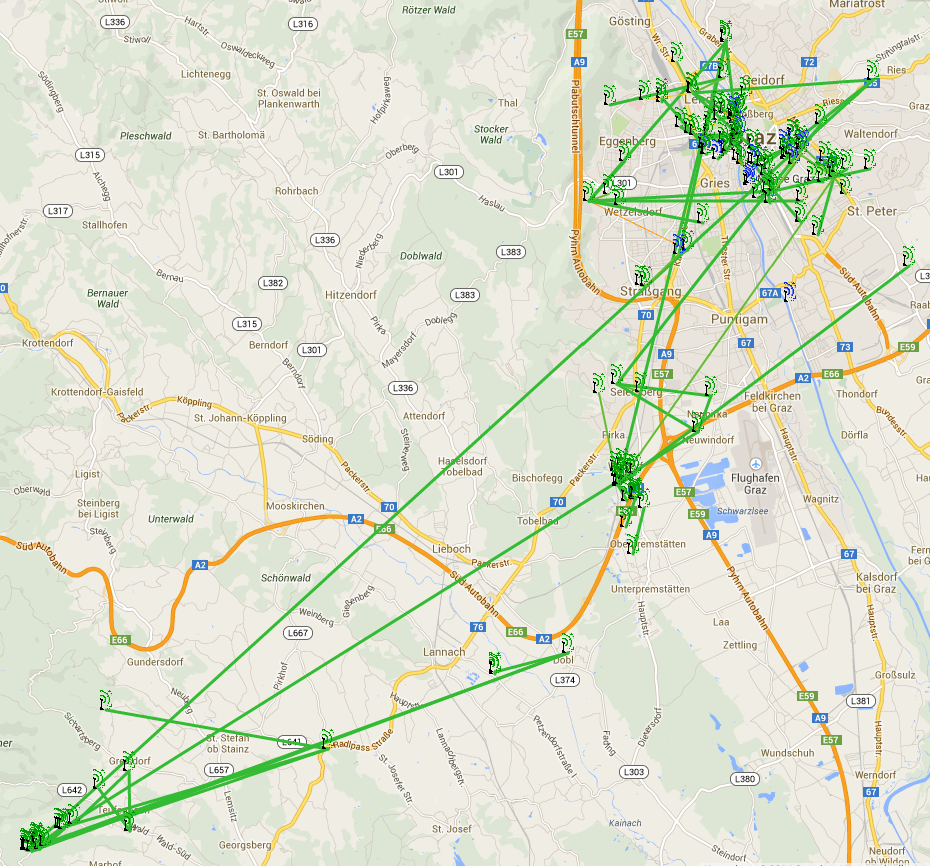
\includegraphics{images/graz_map.png}
  \caption{Map of the FunkFeuer Graz network}
\end{figure}

\clearpage
\section{Comparison}\label{comparison}

\begin{table}
  \centering
  \begin{tabular}{@{}lccc@{}}
    \toprule\addlinespace
    & Ninux & FFWien & FFGraz
    \\\addlinespace
    \midrule
    Nodes & 132 & 237 & 144
    \\\addlinespace
    Links & 154 & 433 & 199
    \\\addlinespace
    Average degree & 2.333 & 3.654 & 2.764
    \\\addlinespace
    Density & 0.018 & 0.015 & 0.019
    \\\addlinespace
    Leaf nodes & 69.02 (52\%) & 77.96 (33\%) & 64.72 (0,45\%)
    \\\addlinespace
    \bottomrule
    \addlinespace
  \end{tabular}
  \caption{High level features of the three WCNs}
\end{table}

\begin{figure}[hbt]
  \centering
  \hspace*{\fill}
  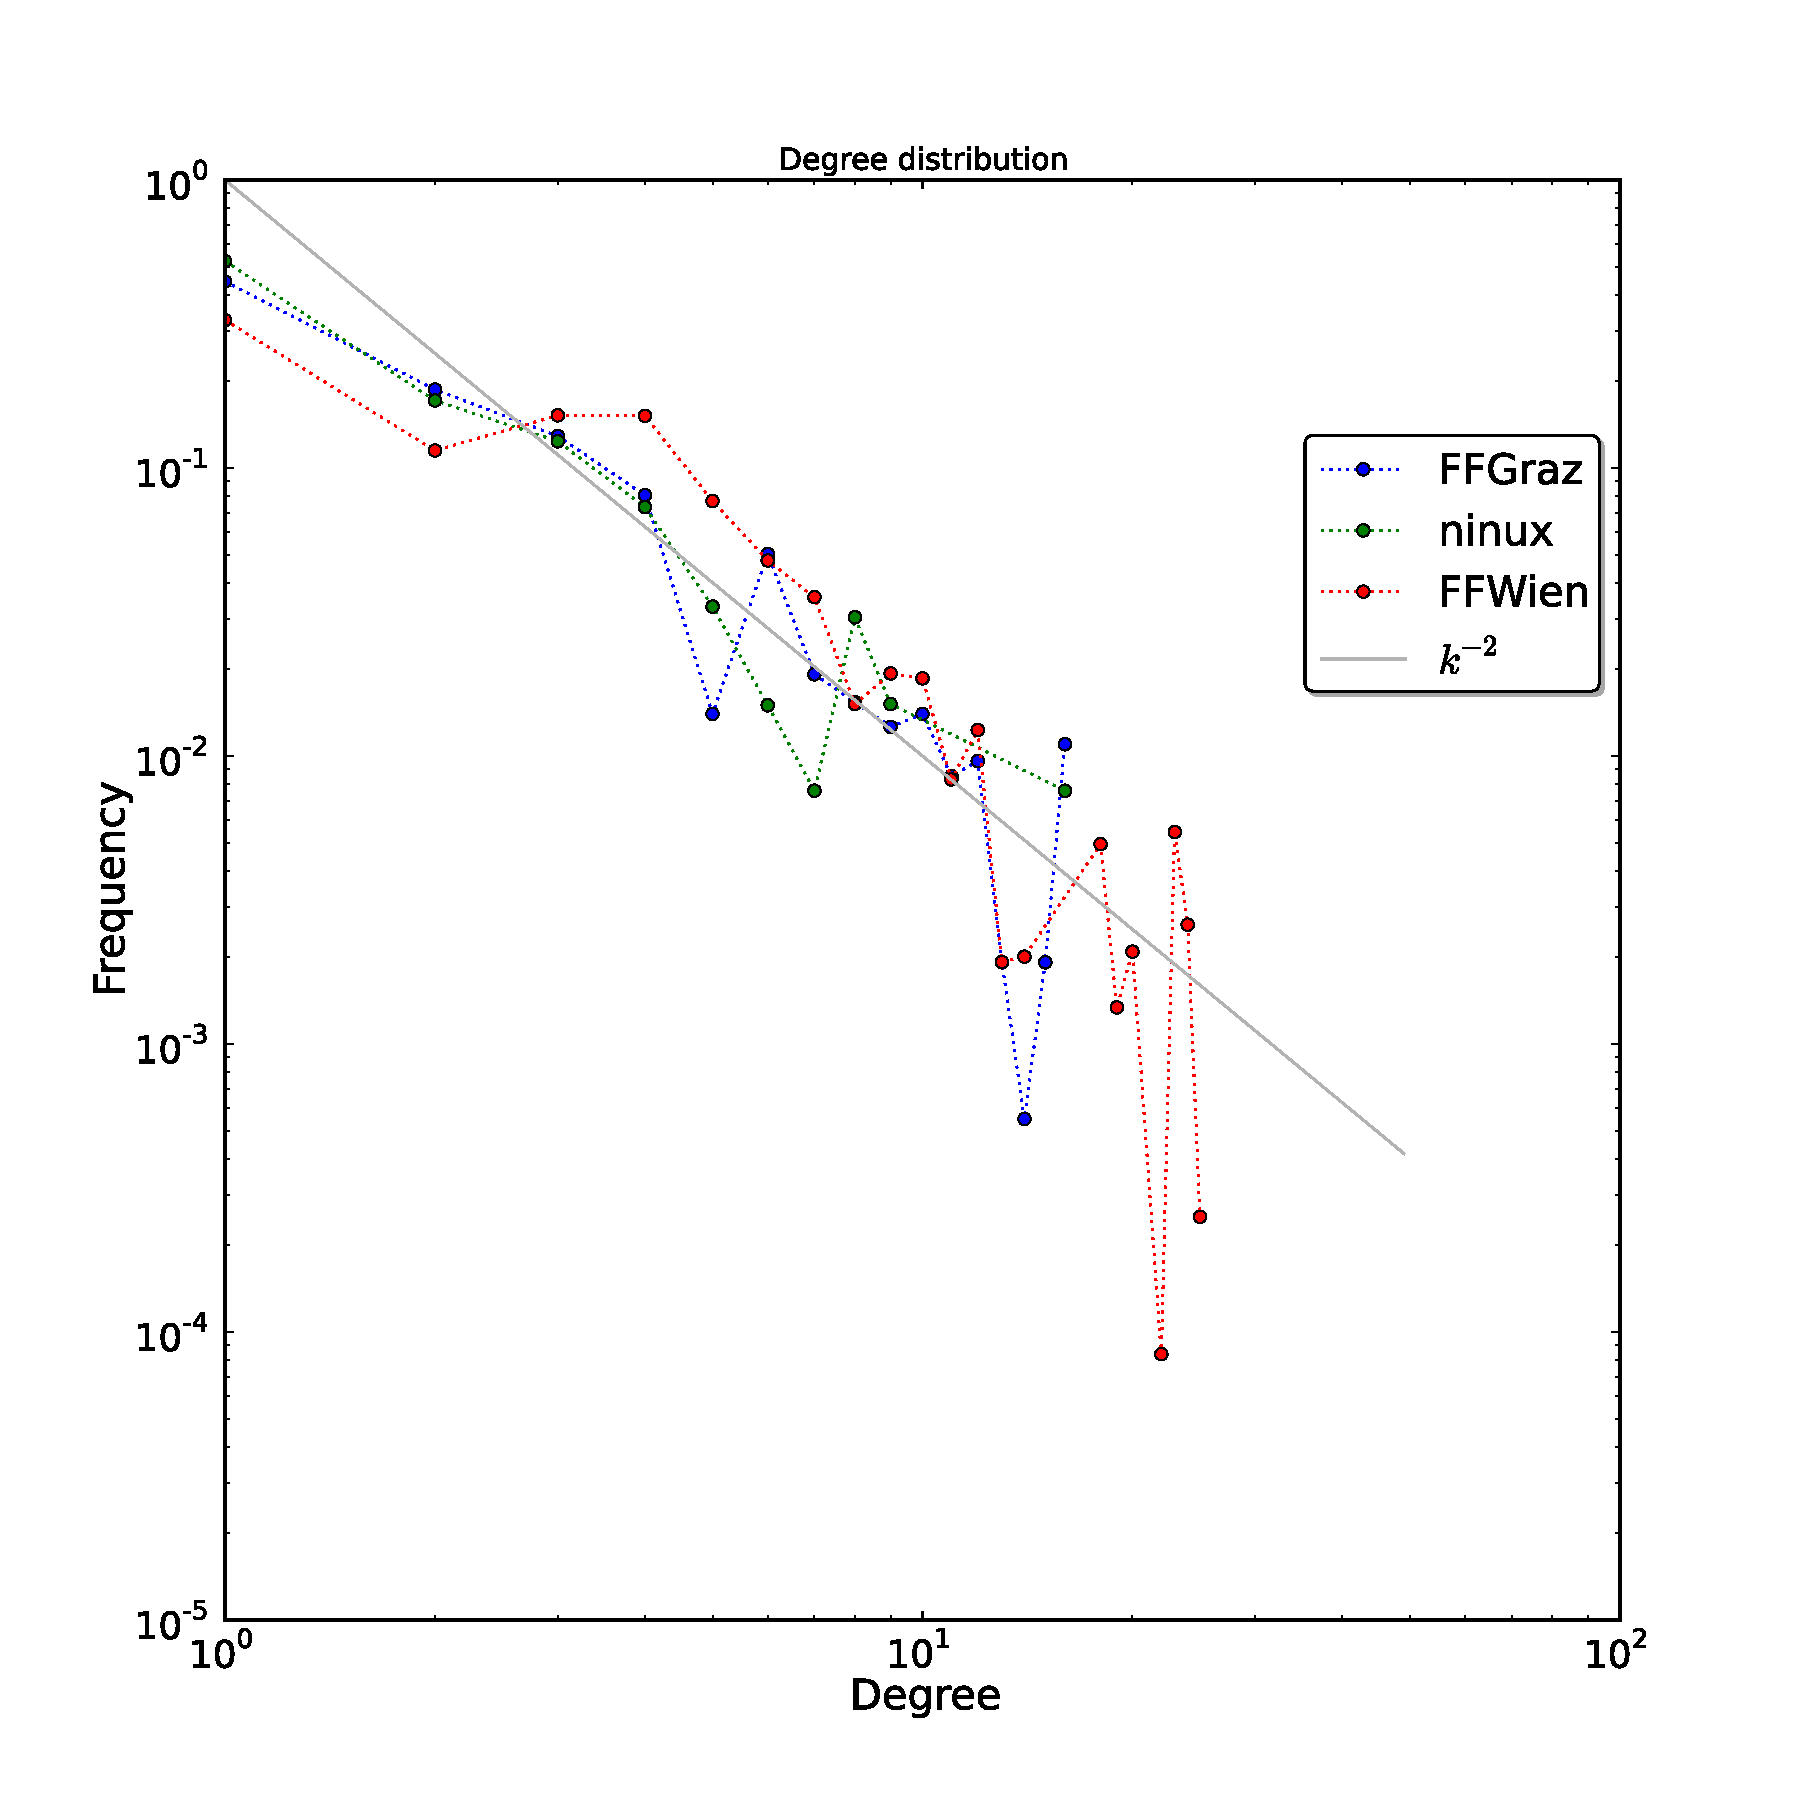
\includegraphics[width=0.49\textwidth]{graphs/degree_distribution_wcn.pdf}
  \hfill
  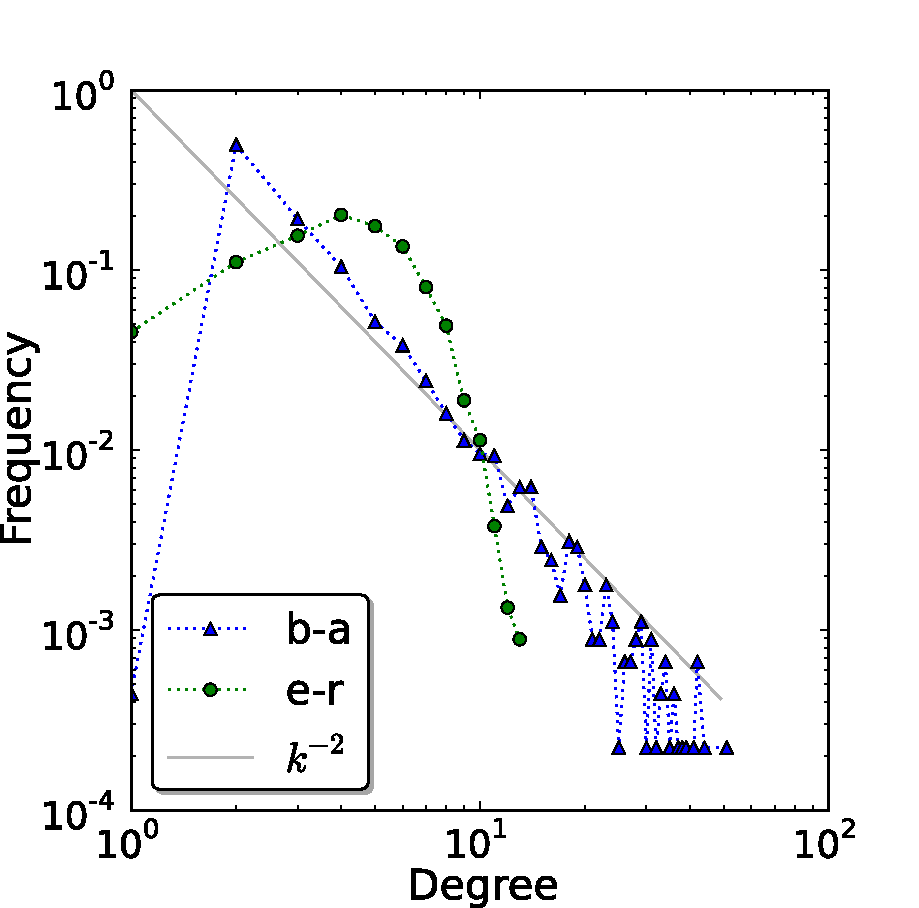
\includegraphics[width=0.49\textwidth]{graphs/degree_distribution_syn.pdf}
  \hspace*{\fill}
  \caption{Degree distribution of the three WCNs, compared with the
    Erd\H{o}s-Rényi and Barabási-Albert models}
  \label{fig:wcn-degree-distribution}
\end{figure}

As \figref{fig:wcn-degree-distribution}
shows, the degree distributions of the three WCNs
roughly follow a power law $k^{-2}$, as does the random Barabási-Albert
model. One objective of this analysis is to understand if the model can
be used to predict other properties of the real networks.

\begin{figure}[htb]
\centering
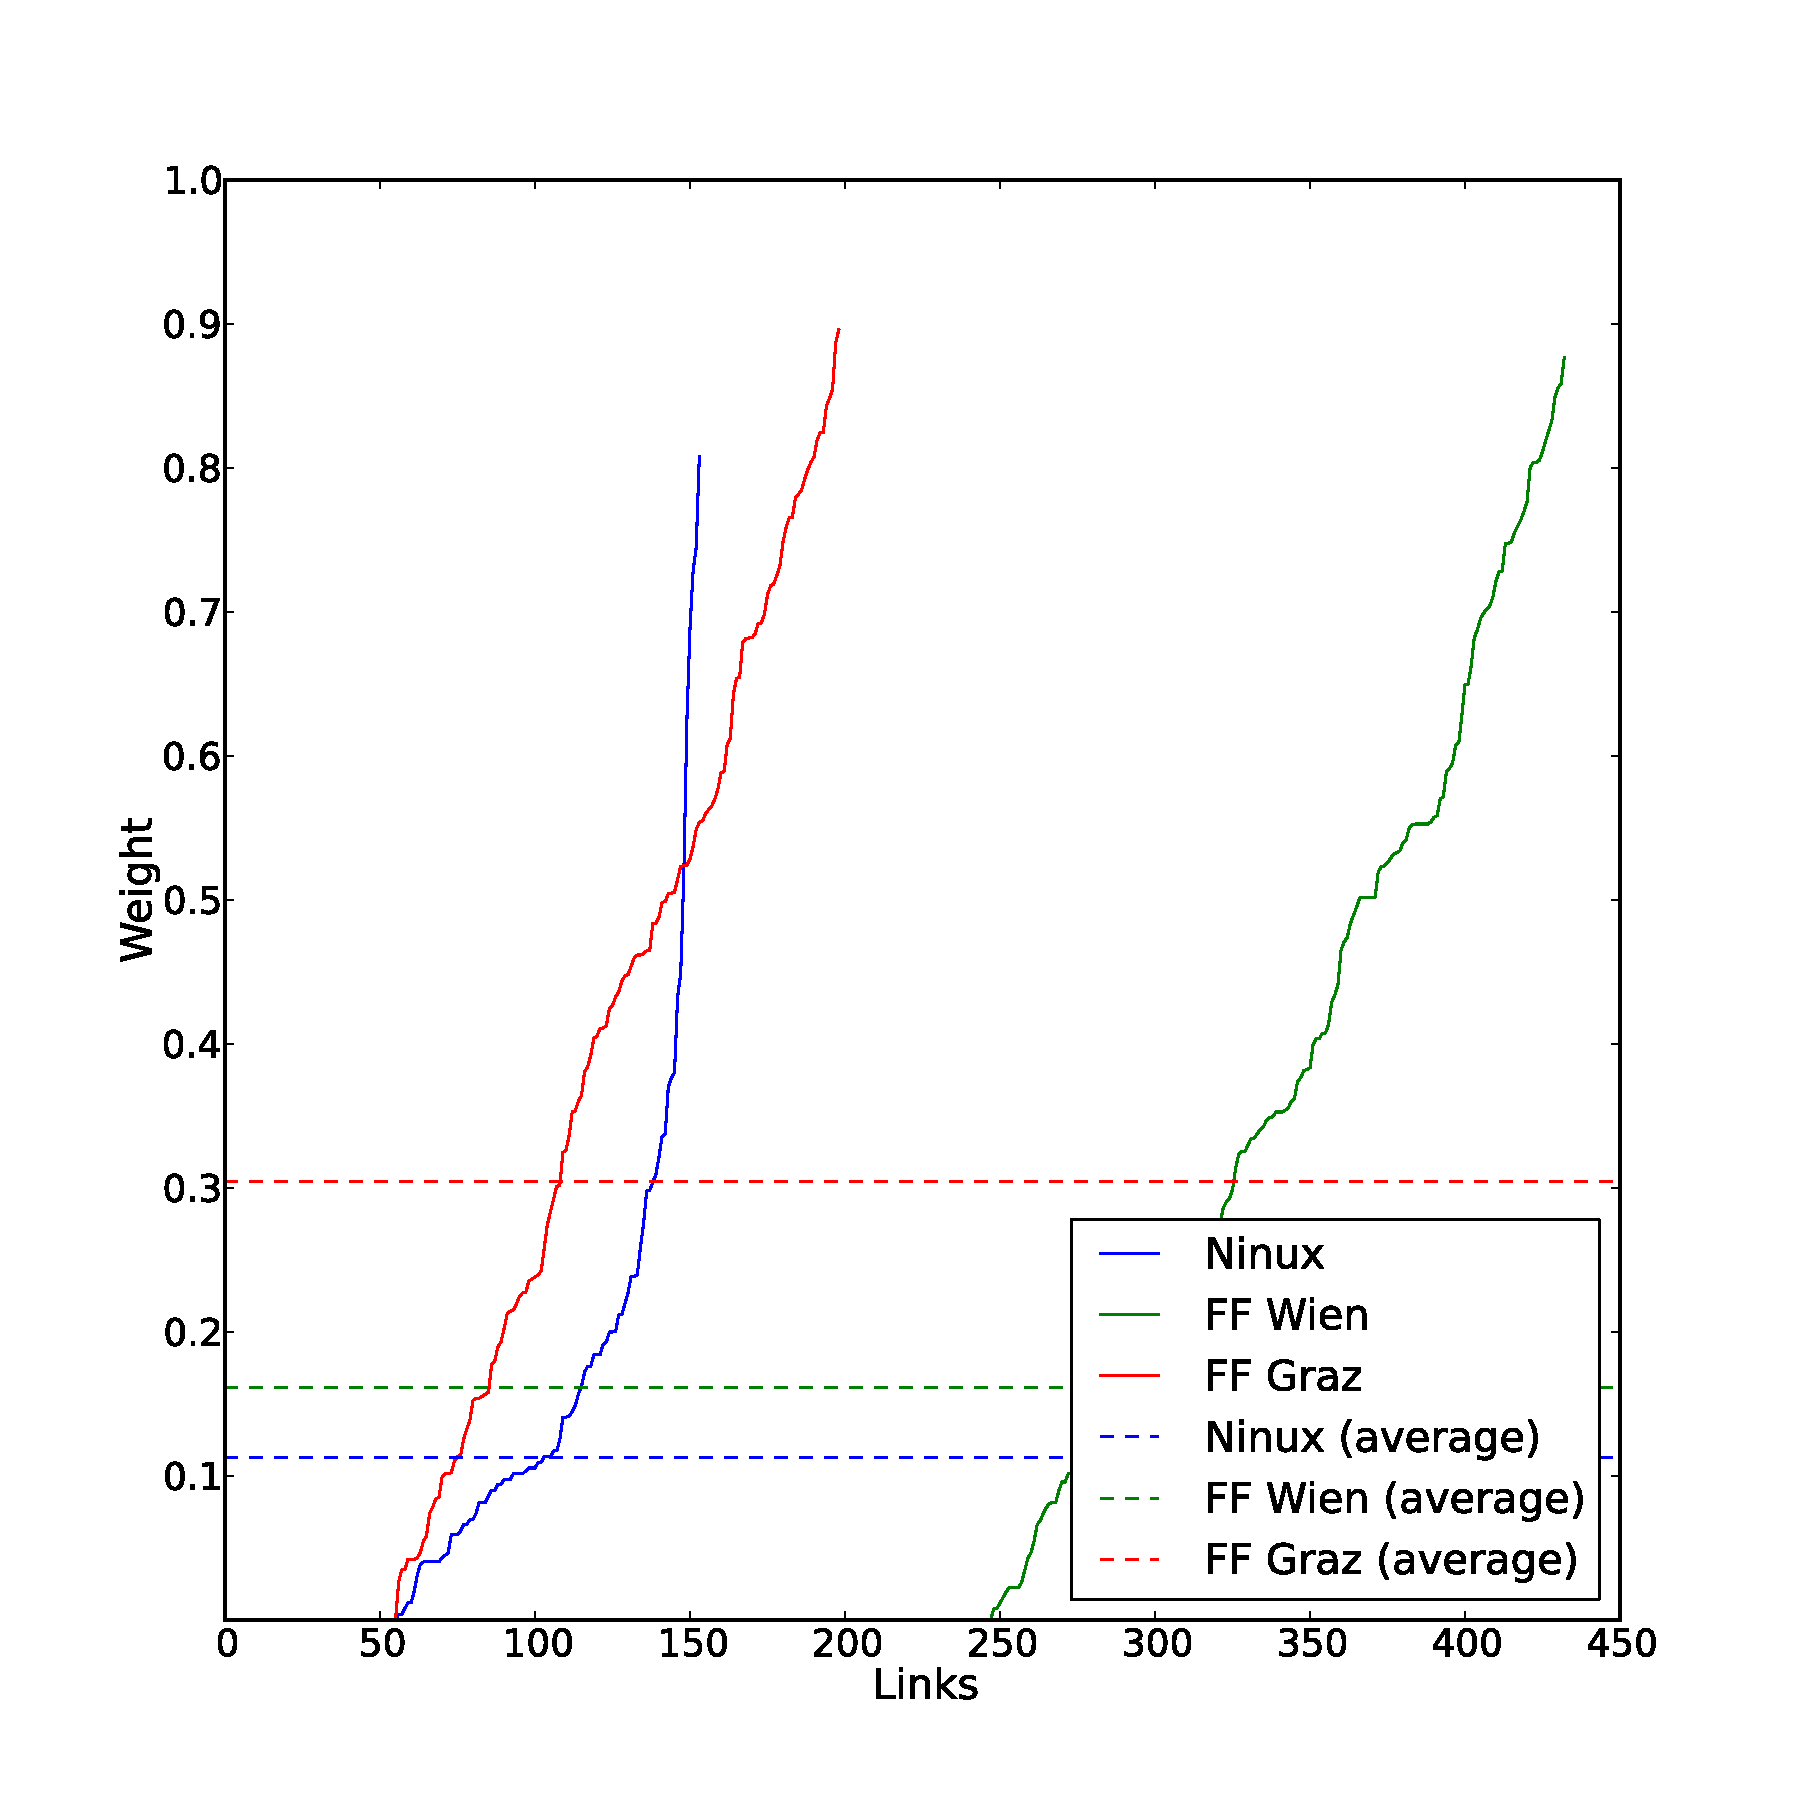
\includegraphics{graphs/weight_rank.pdf}
\caption{Links of the three WCNs, ranked by probability to lose packets}
\label{fig:wcn-link-ranking}
\end{figure}

As can be seen in \figref{fig:wcn-link-ranking}, the three networks have a quite
different distribution of link quality (the metric shown in the graph is
$1 - \frac{1}{\etx}$, which is also used for the signalling analysis in
\hyperref[message-propagation-analysis]{chapter 5}). FunkFeuer Graz has by far the highest average
weight, while Ninux seems to have the best links.

\chapter{Robustness analysis}\label{robustness-analysis}

The first metric analysed is the robustness of the network. The chosen
methodology is a variation of the percolation process described in
Chapter 16 of (Newman 2010).

\section{Percolation}\label{percolation}

Percolation is the process of removing nodes (\emph{site percolation})
or edges (\emph{bond percolation}) and observing the properties of the
remaining graph. More specifically, by examining the connected
components of the graph, it can be decided if the underlying system is
still functioning the same after removing nodes (or edges). The removal
of nodes simulates a variety of real-world situations -- from hardware
failures in communication networks to vaccinated people in the spread
of a disease. Removing edges addresses other cases, also interesting in
real-world systems. In the following paragraphs, only site percolation
is considered, but the remarks are also valid, with the necessary
adaptations, for bond percolation.

It is not trivial, at a first look, how it should be decided if the
network ``functions'' after removing nodes. Nonetheless, there is a
simple answer to this issue that gives very significant results: the
order of the largest connected components. Removing a node from a
network obviously removes the node itself from any connected component,
but also affects potentially other nodes, which received information
through the removed node.

If enough nodes are removed, the network will become disconnected, but
usually there will be a large connected component containing most of the
surviving nodes and some smaller ones with just a few nodes. It can be
affirmed that in such a situation, at least part of the network is still
working as intended. Removing even more nodes, however, leads to a point
where the largest component does not contain a significant fraction of
the nodes -- it becomes indistinguishable from the smaller ones. This is
the point in which the network loses all its function.

To formally define a robustness metric, name the connected components of
a graph, ordered non-increasingly by the number of their nodes,
$C_0, \ldots, C_m$. $|C_0|$ is then the order (number of nodes) of the
largest connected component. The robustness metric is defined as

\begin{equation}
S = \frac{|C_0|}{|V|}
\end{equation}

\section{Removal order}\label{removal-order}

Nodes and links in a network are not all equal. As seen in
\hyperref[network-topology-and-graphs]{Chapter 3}, different
centrality metrics give different measures of the importance of a node
in a network. When considering robustness, it is interesting to study
which nodes have the biggest impact when removed and how much difference
there is between more and less impacting nodes.

The classical approach to percolation is to remove nodes randomly in an
uniform way. Also popular is the removal of the nodes with highest
degree first. Other methods, such as ordering by centrality, have also
been explored. Comparing this different methods gives not only useful
information on how the metrics predict the impact of a node when
removed, but also on the behaviour of the examined networks. Some
networks, for example, behave more or less the same regardless of the
order of removal. Others show a dramatically different response.
Scale-free networks are the typical example of a network that is highly
robust to random failures, but collapses quickly if the nodes with the
highest degree are removed.

Changing the removal order has also another level of significance when
studying real-world networks. There are various situations in which
nodes have different probabilities of failing: for example, malicious
attacks often try to target the nodes that would cause the most damage.

All of the above considerations are also valid for links, but the
metrics differ: there is nothing corresponding to the degree, but there
is betweenness centrality.

This analysis covers random removal of both nodes and links, removal of
links by betweenness centrality and of nodes by degree, betweenness and
closeness centrality.

\section{Comparing different networks}\label{comparing-different-networks}

The objective of doing a robustness analysis on WCNs, apart from
determining their resilience to failure, is also understanding if the
presently used random models are useful in describing their behaviour.

One feature of networks that highly influences their robustness is the
density of links with respect to nodes. Intuition suggests that a
network with more links should be more robust of a less dense one with
the same number of nodes. This is in fact confirmed.

Keeping this in mind, any robustness comparison between two networks is
significant if the networks have comparable densities. It is of no use
comparing a 100-node network with 200 edges to one with 2000.

To express the density of a graph, the average degree may be used.
Recall the three WCNs which are the subject of this analysis have
average degrees 2.333, 3.654 and 2.764. Since they are to be compared to
graphs generated by random models, care must be taken to generate graphs
with an average degree not too distant from those.

The average degree of random graphs can be predicted easily, given the
parameters:

\begin{itemize}
\item
  for the Erd\H{o}s-Rényi $G(n,p)$ model, the expected average degree is

  \begin{equation}
  \left< k \right> = \frac{2 \binom{n}{2} p}{n} = (n-1)p
  \end{equation}
\item
  for the Barabási-Albert preferential attachment model the exact
  average degree is known

  \begin{equation}
  \left< k \right> = \frac{2 (n-m)m}{n} = 2m\left( 1 - \frac{m}{n} \right)
  \end{equation}
\end{itemize}

Unfortunately, while the $p$ parameter of the $G(n,p)$ model is a real
number and can be adjusted at will, the preferential attachment models
requires a natural number $m$. This means that only some values of
average degree can be achieved.

\begin{longtable}[c]{@{}ccccccc@{}}
\toprule\addlinespace
$m$ & 1 & 2 & 3 & 4 & 5 & 6
\\\addlinespace
$\left< k \right>$ & 1.99 & 3.96 & 5.91 & 7.84 & 9.75 & 11.64
\\\addlinespace
\bottomrule
\addlinespace
\caption{Average degrees for a 200-node graph with the Barabási-Albert
model}
\end{longtable}

\section{Methodology}\label{methodology}

The analysis was performed on 50 snapshots of the topology of the three
WCNs, as well as 30 graphs for each of the random models.

The algorithm simply removed nodes (or links) one by one and checked the
size of the largest connected component. In the case of random removal,
the test was repeated 30 times for each graph, changing the order every
time.

The test considered the removal of at most 40\% of the nodes (or links).
Other values have been tried, but this was determined to be sufficient
to observe the expected behaviour. Highest values just increased the
simulation time without adding useful information.

The results were averaged over the graphs of the same kind and expressed
in term of fraction of removed nodes, rather than number of nodes, in
order to compare them in the same graph.

\section{Results}\label{results}

\begin{figure}[htbp]
\centering
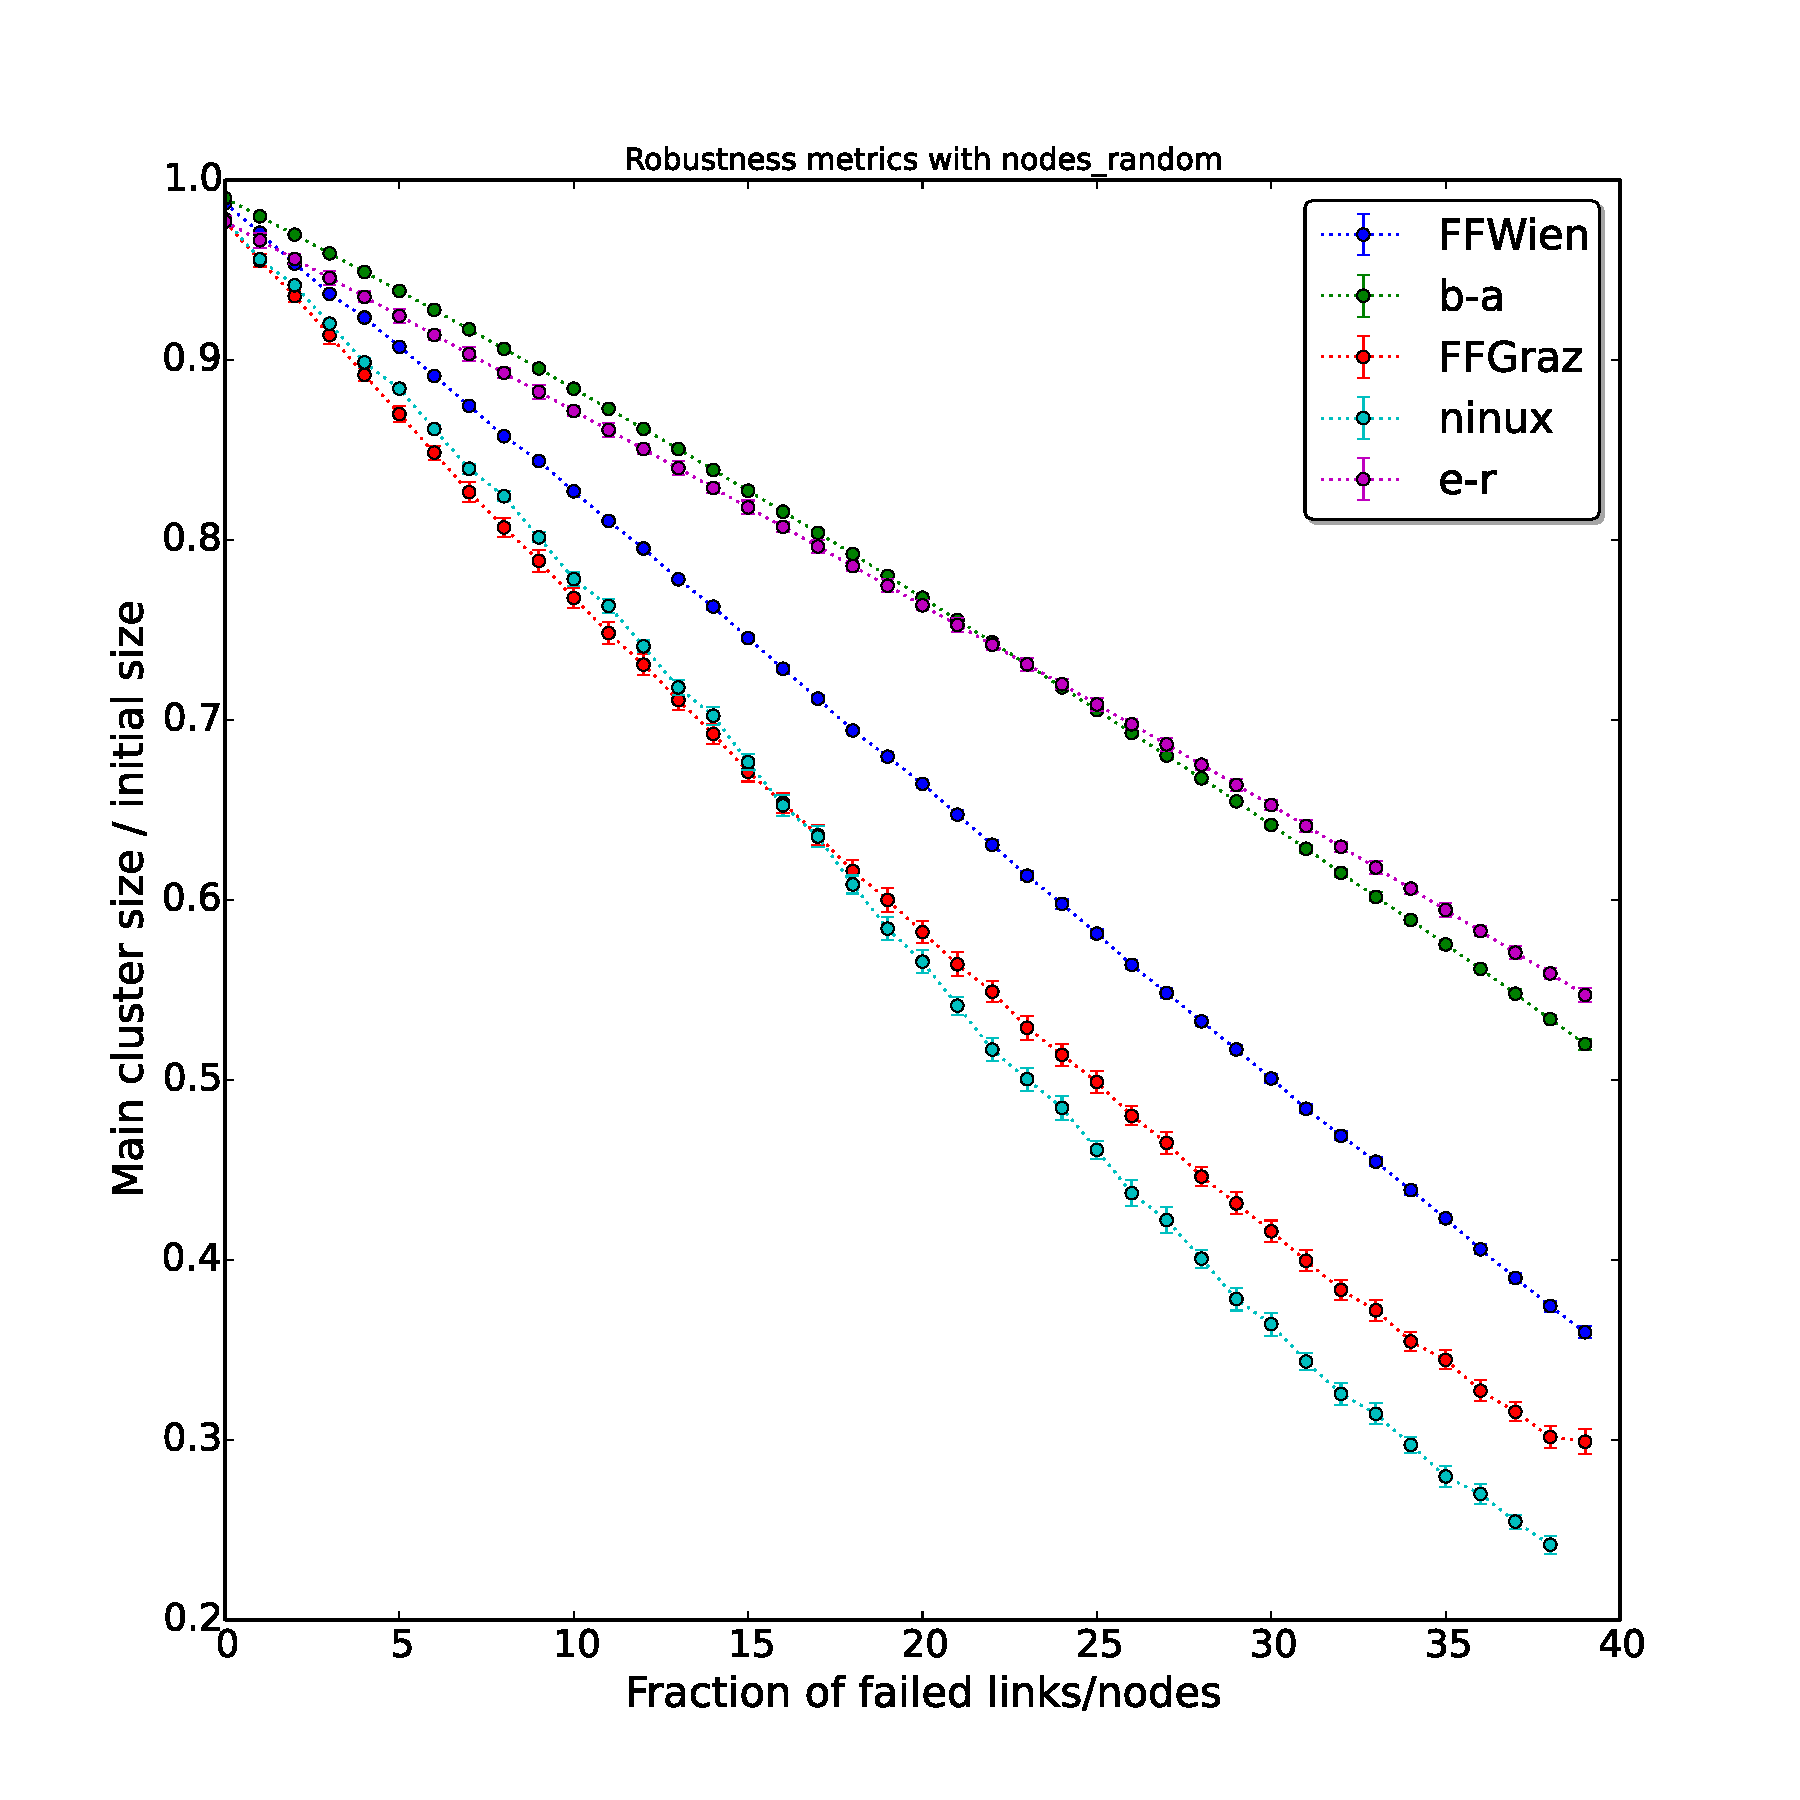
\includegraphics{graphs/nodes_random_robustness}
\caption{Random removal of nodes}
\label{fig:node_rand}
\end{figure}

\begin{figure}[htbp]
\centering
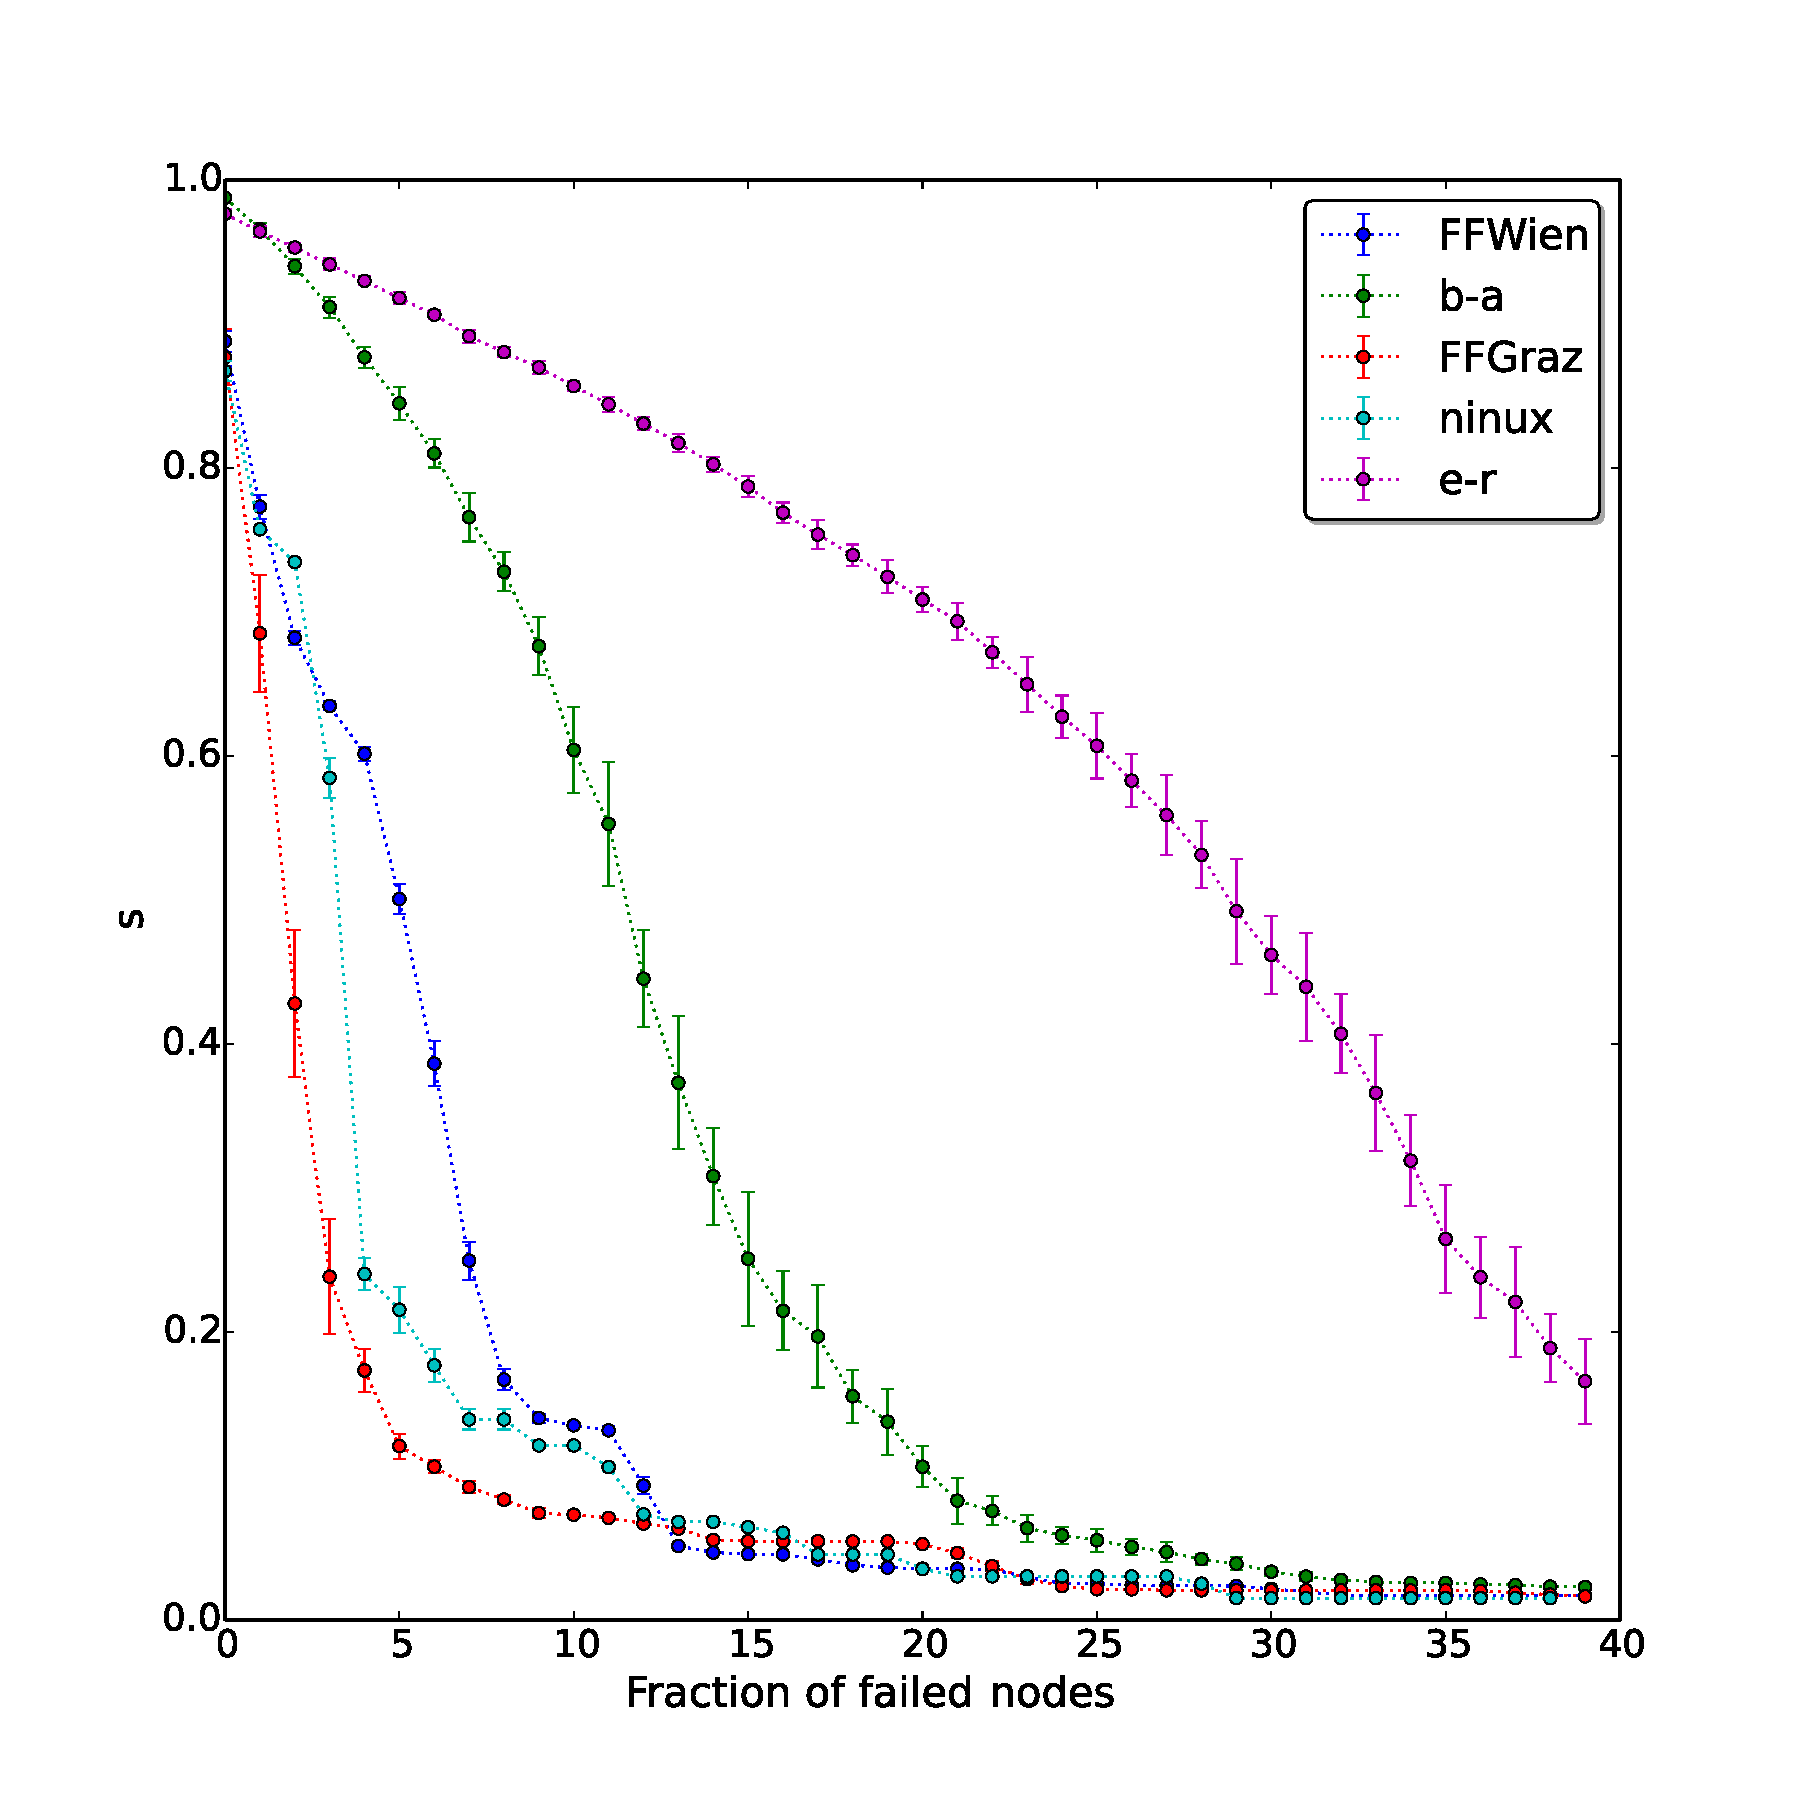
\includegraphics{graphs/nodes_deg_robustness}
\caption{Removal of nodes by degree}
\label{fig:node_deg}
\end{figure}

\begin{figure}[htbp]
\centering
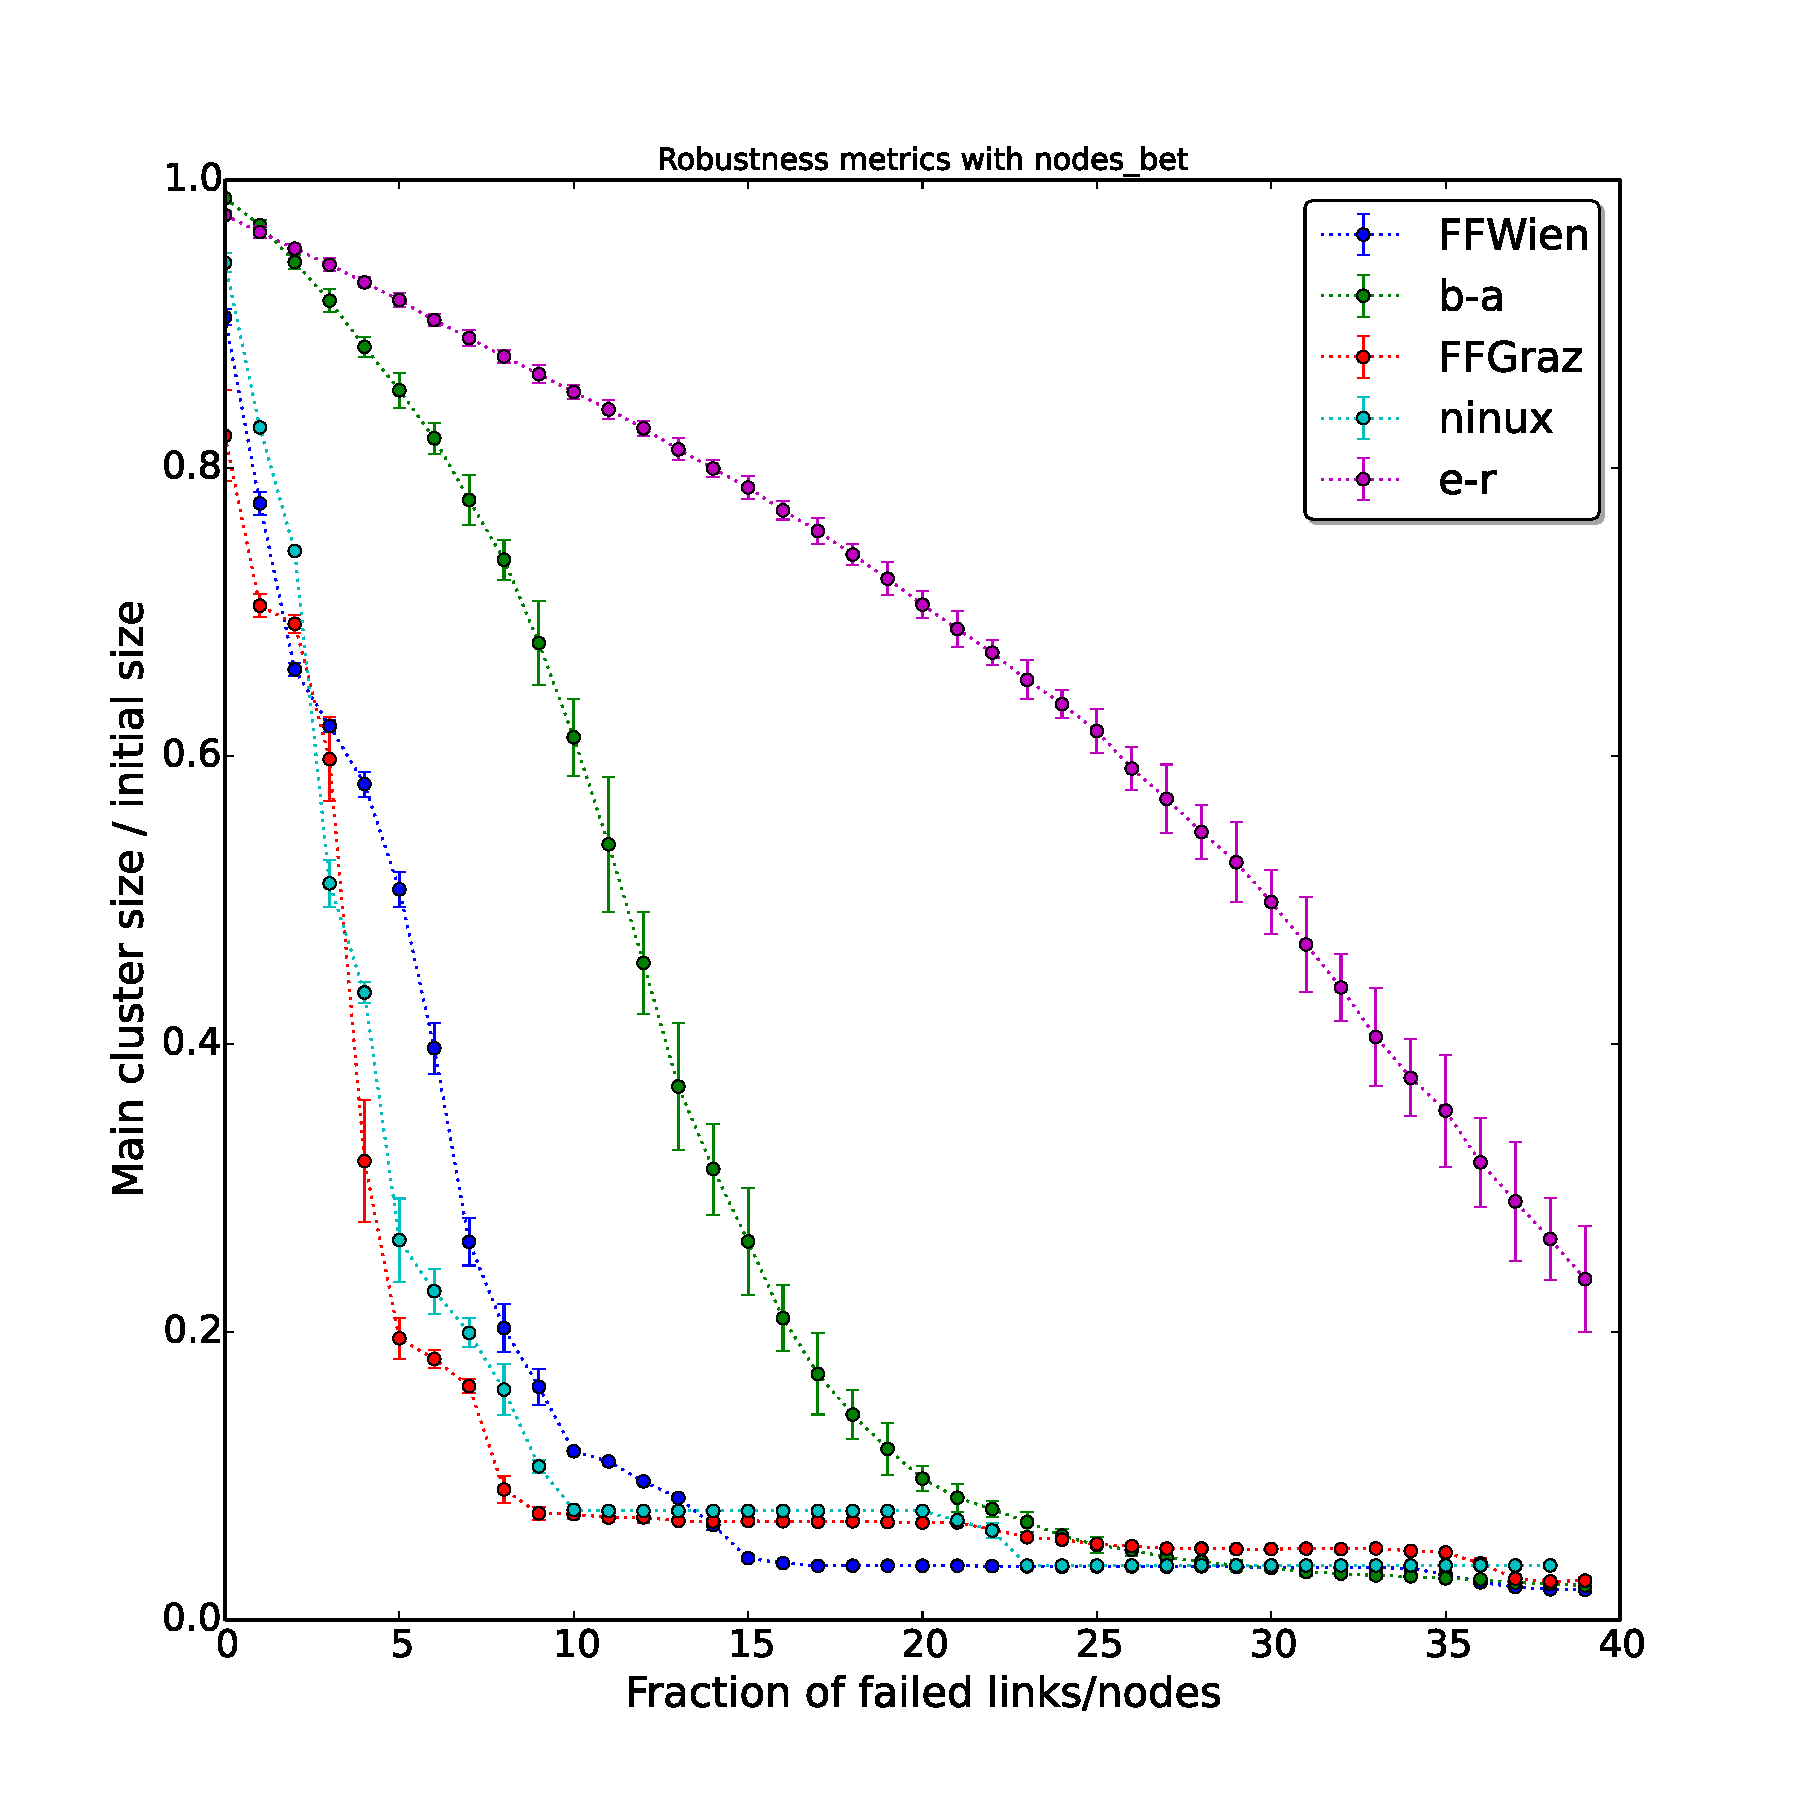
\includegraphics{graphs/nodes_bet_robustness}
\caption{Removal on nodes by betweenness centrality}
\label{fig:node_bet}
\end{figure}

\begin{figure}[htbp]
\centering
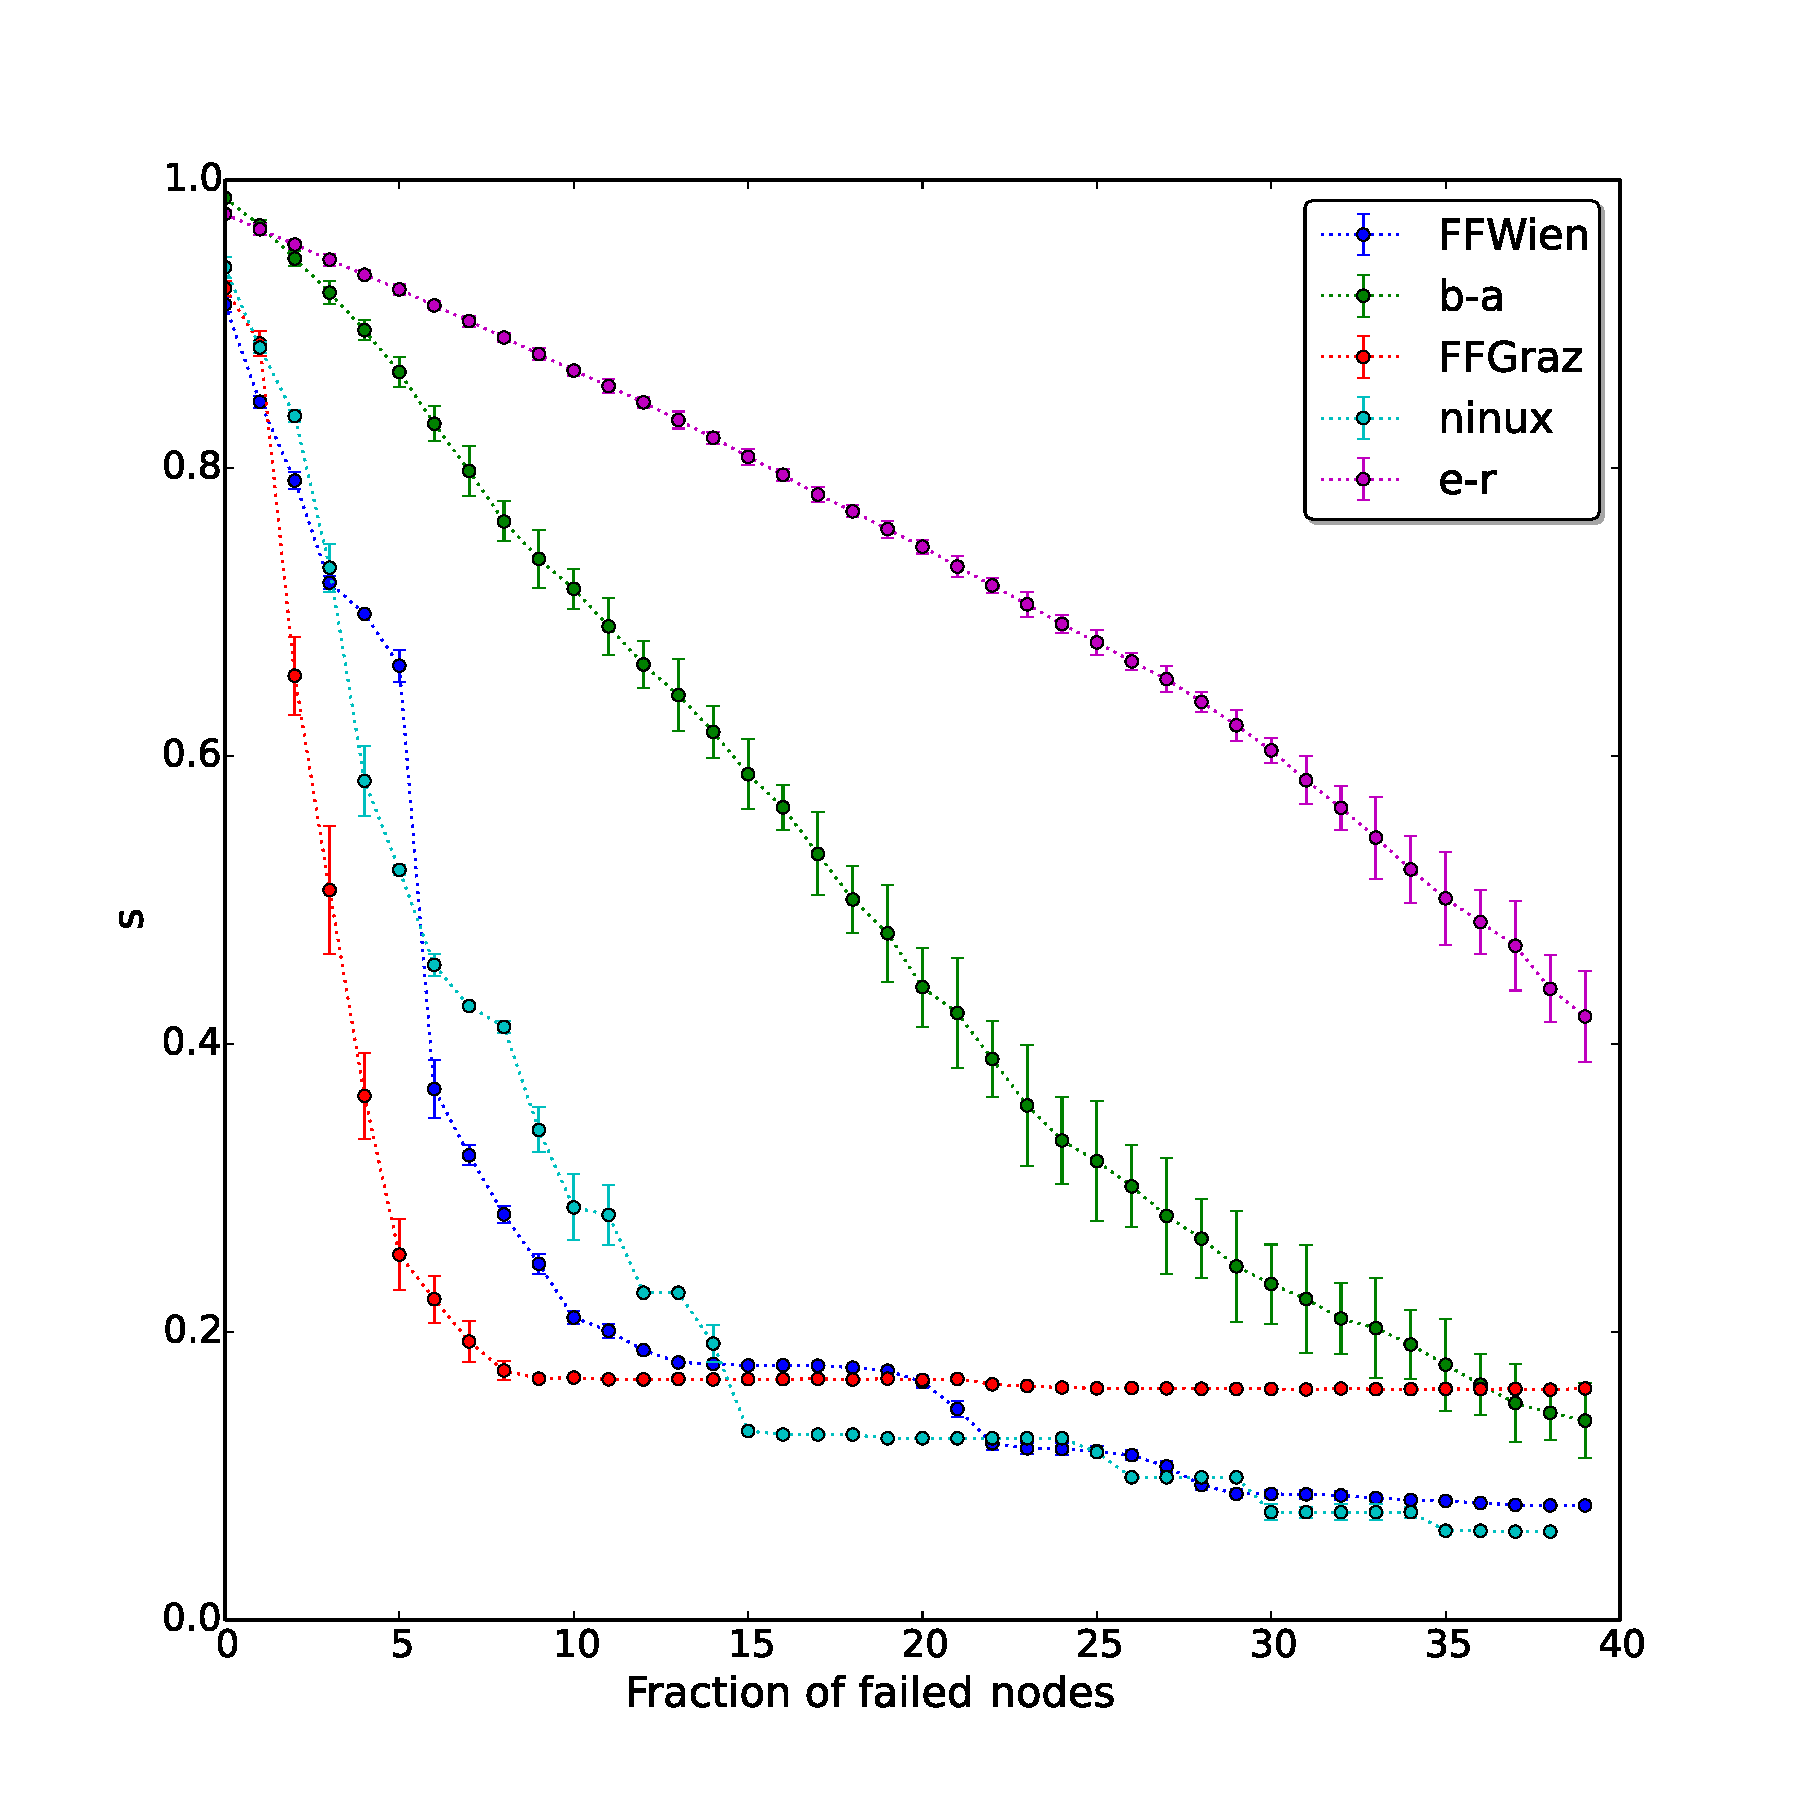
\includegraphics{graphs/nodes_close_robustness}
\caption{Removal of nodesby closeness centrality}
\label{fig:node_close}
\end{figure}

\begin{figure}[htbp]
\centering
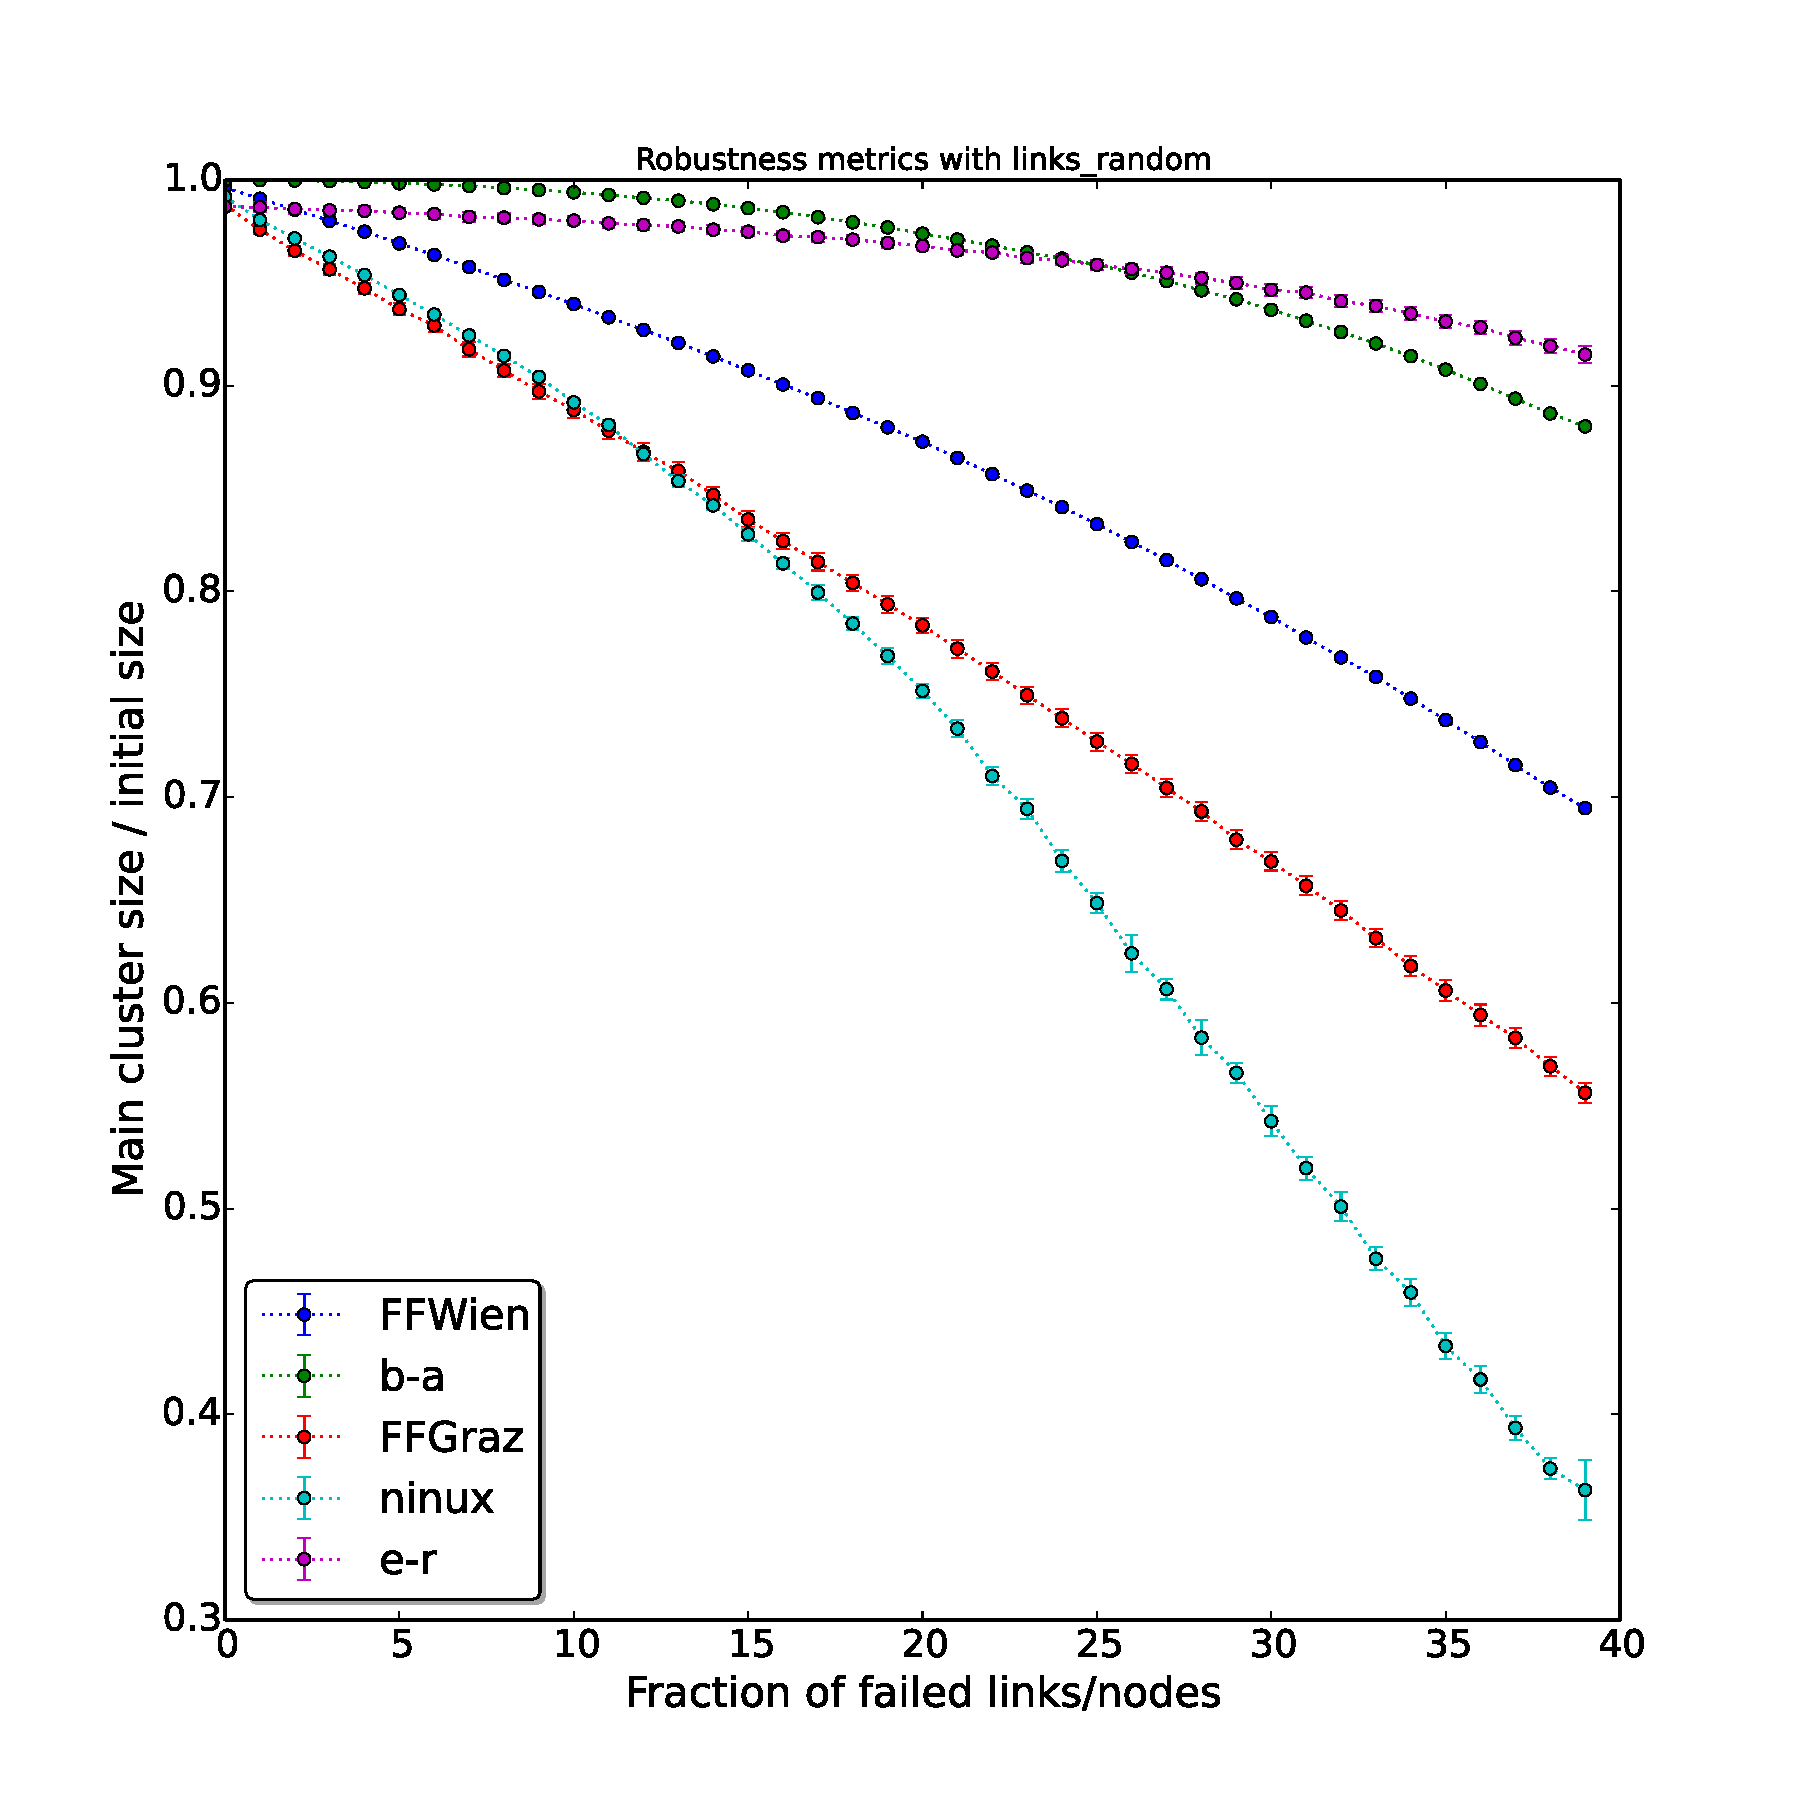
\includegraphics{graphs/links_random_robustness}
\caption{Random removal of links}
\label{fig:link_rand}
\end{figure}

\begin{figure}[htbp]
\centering
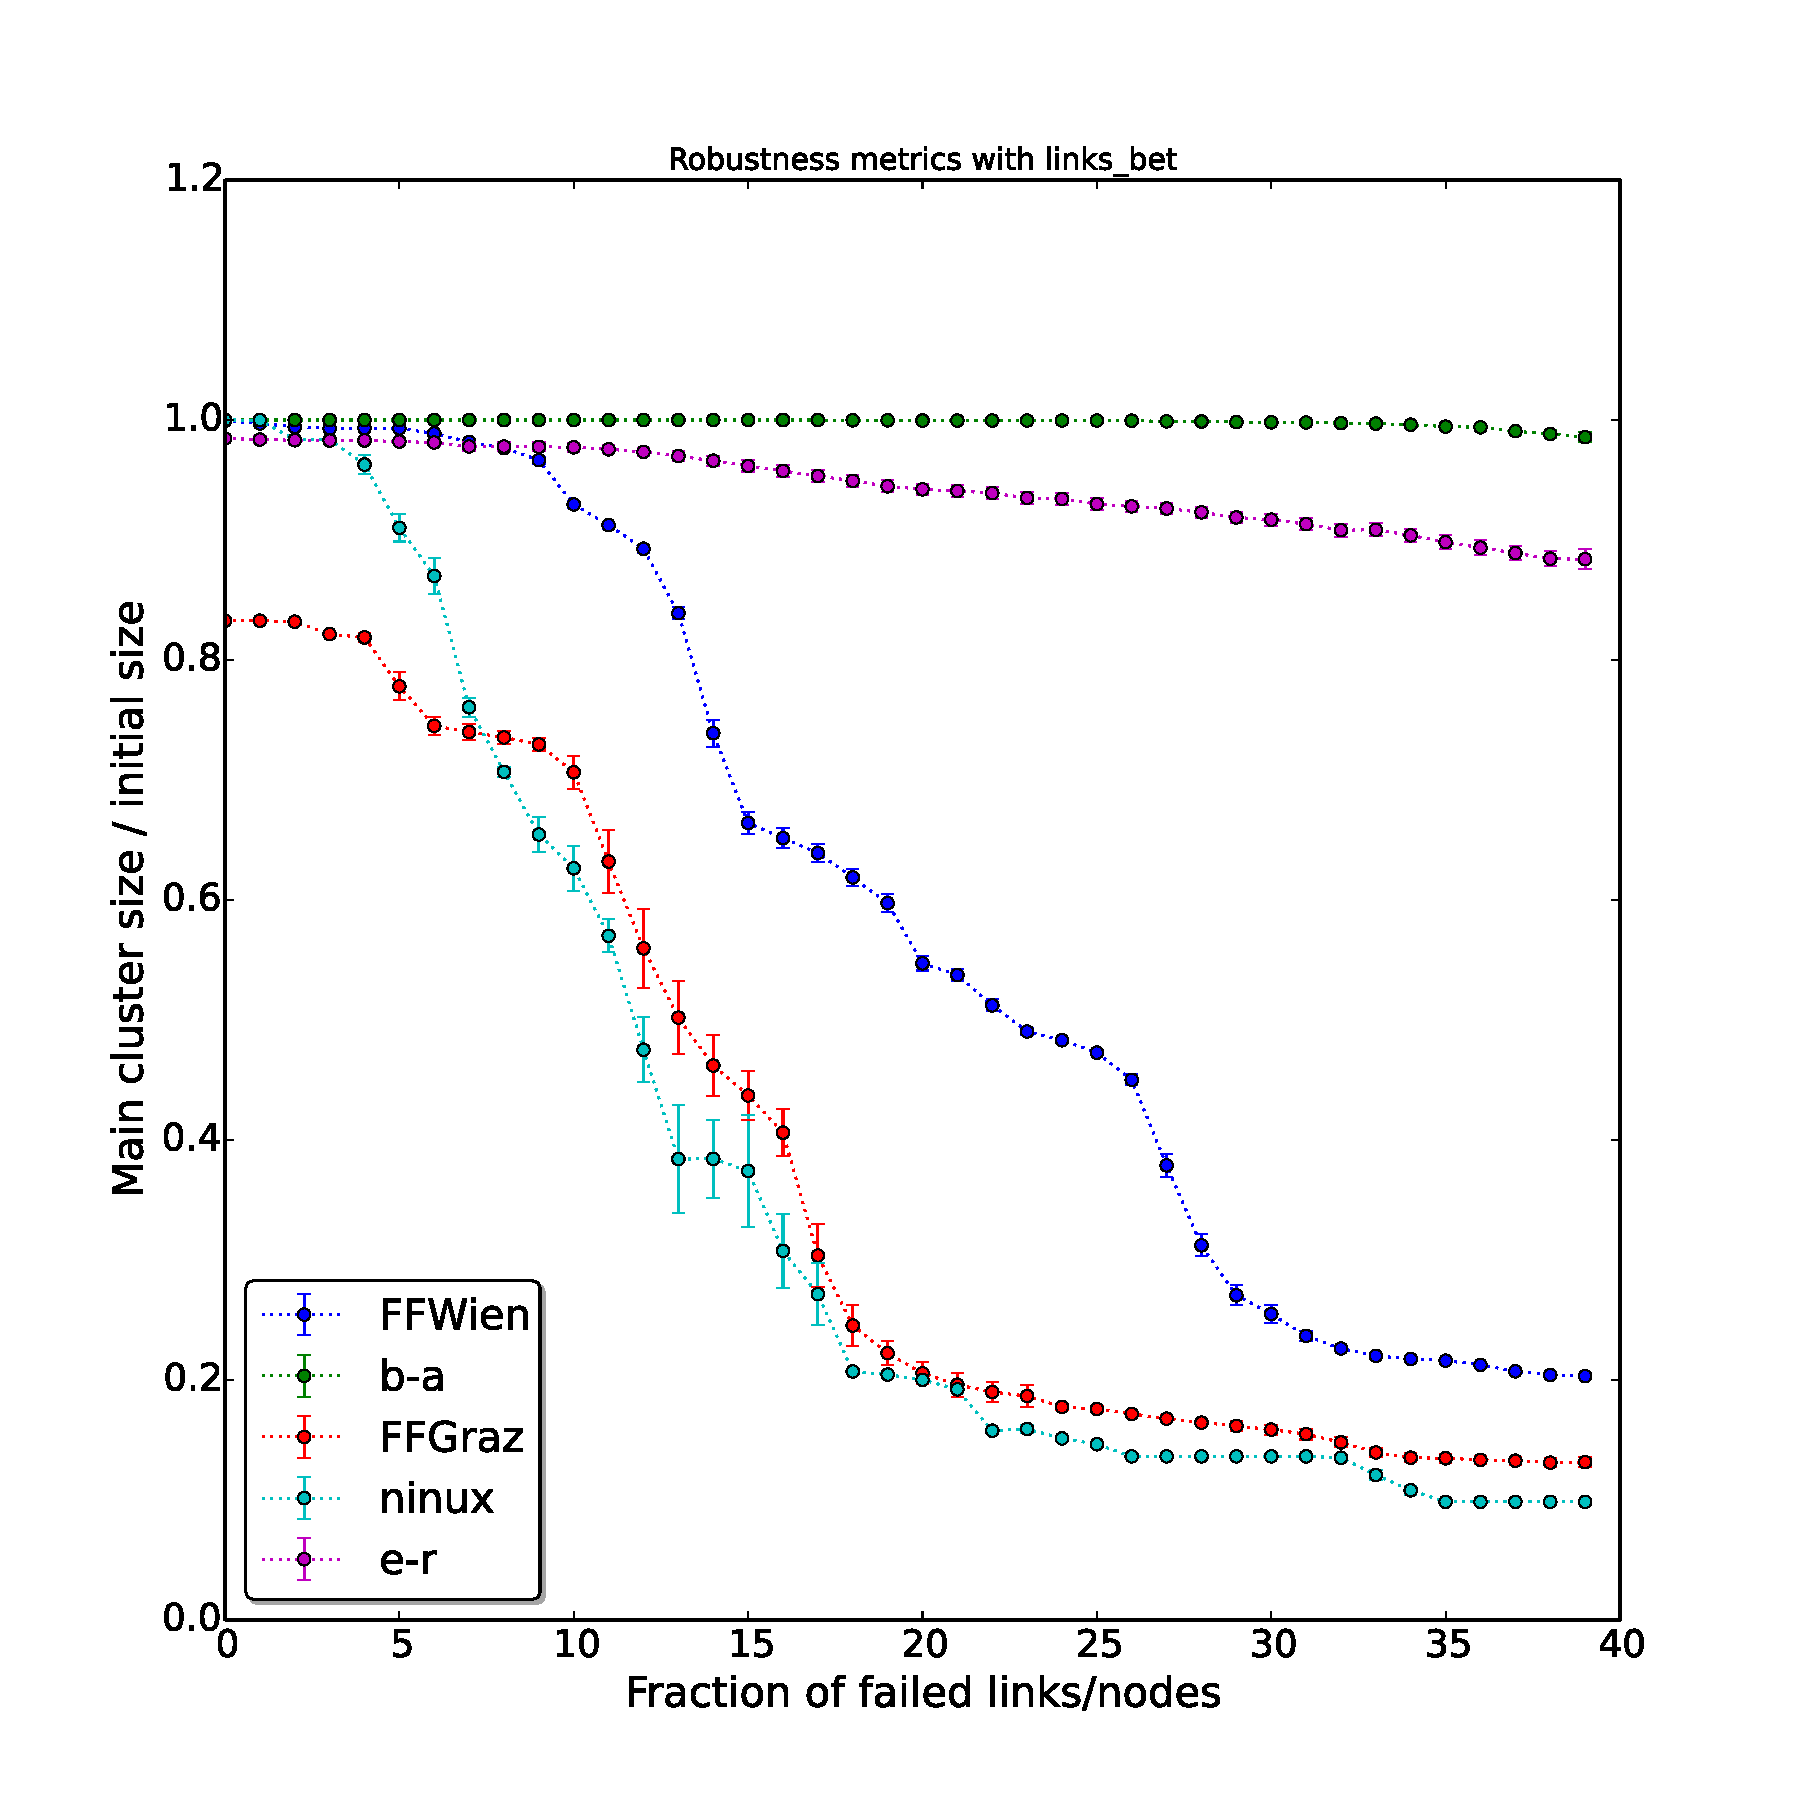
\includegraphics{graphs/links_bet_robustness}
\caption{Removal of links by betweenness centrality}
\label{fig:link_bet}
\end{figure}

As shown in the figures, there is a marked difference between the
behaviour of the three WCNs (which is similar) and the behaviour of the
random graphs. The WCNs are more fragile in all tests, but while the
difference in the random removal case (\figref{fig:node_rand}) may be
explained by the lower density, in all of the ordered removal cases they
consistently fail after just 10\% of nodes are removed.

The scale-free random networks is, as expected, less robust than the
Erd\H{o}s-Rényi model in targeted attack to nodes with the highest
degree (\figref{fig:node_deg}), and has the same proceeding with removal
by betweenness (\figref{fig:node_bet}). On the
other hand, removing nodes by closeness centrality (\figref{fig:node_close})
shows a quite less marked difference between the two models.

WCNs, on the contrary, behave the same in all the scenarios in which
nodes are removed in order, independently from the metric used
(\figref{fig:node_deg}, \ref{fig:node_bet}, \ref{fig:node_close}). This
suggest that, in those networks, the central nodes are the same for all
the metrics. This also means that the topology of WCNs, despite the big
similarity of the degree distribution, is different from the
preferential attachment model. Moreover, this difference seems to go in
the direction of less robustness.

The removal of links (\figref{fig:link_rand} and \ref{fig:link_bet})
also shows a similar picture. None of the random
models approximates well the behaviour of the WCNs, which quickly fail
after a small fraction of links has been removed. Here a peculiar
behaviour appears in FFGraz: in this network, there are some nicely
connected areas that are geographically distant between themselves, so
there are some long links that provide connection between those
clusters. These long links are apparently (and intuitively) the ones
with the highest centrality, so the first to be removed.

The inadequacy of the preferential attachment model to predict the
robustness of WCNs deserves some considerations. Despite the degree
distributions following in both cases a power law, the robustness
metrics behave quite differently, so it is worth considering what are
the features of real world networks the model does not account for.

Firstly, one thing that can be noticed is that the preferential
attachment model builds a graph with no leaves. With $m = 2$, which is
the parameter used in this analysis, the graph at step zero is two
vertices without links, at step 1 it is a path of length 2, at step 2 it
is either a square or a triangle with a leaf.
In either case, since each new node is added with 2 links, the final
graph will contain at most 1 leaf, in contrast with WCNs where leaves
are a large part of the nodes.

A second observation is that the nodes with highest degree in WCNs
are usually those installed in good locations (for instance on a hill
or another elevated spot). This is because Wi-Fi links require a line
of sight.
When a new node is added it usually starts as a leaf and does not choose
its neighbour(s) based on their degree, instead it is forced to choose
a node it can see.
So, the growth of a WCN does not follow the preferential attachment rule,
even if the resulting degree distribution seems similar.

\chapter{Message propagation analysis}\label{message-propagation-analysis}

\section{The importance of signalling}\label{the-importance-of-signalling}

The robustness of a network is based on a static analysis of the
connectivity of the network graph when removing nodes or links. A
communication network, however, is a dynamic system where information
needs to move between nodes. Moreover, the decentralised nature of
computer networks means that the complete topology of the network is not
necessarily the topology used to transmit information, depending on the
routing protocol used for the network.

Given this, in order to understand the behaviour of a communication
network it is necessary to study the behaviour of its routing protocol
with different underlying topologies. The phase analysed here is that of
topology discovery, where link-state advertisements are exchanged and
each node receives information on the existence of the other nodes in
the network and a route to reach them.

In traditional link-state routing protocols, link-state advertisement
messages are usually flooded through the network with a simple duplicate
detection mechanism to avoid broadcast storms.

OLSR uses a more sophisticated technique to reduce the overhead of
routing. This of course comes at a cost in redundancy, since if a link
loses \texttt{TC} messages, these are not received through other routes.
OLSR also has \texttt{HELLO} messages, which are only exchanged with
neighbours and allow \texttt{TC} messages, which are only generated by
MPRs, to contain information about all the neighbours of the node which
generates them.

The implementation of OLSR used in WCNs differs from the specification
and forgoes optimization by forcing each node to be an MPR.

All of this three variants of signalling have been simulated on the
topologies of the analysed networks, thus having:

\begin{itemize}
\itemsep1pt\parskip0pt\parsep0pt
\item
  simple flooding of messages with information on the sender node only
  (L-S)
\item
  simple flooding of messages with information on the sender and its
  neighbours (WCN)
\item
  optimized flooding (with MPRs) of messages with information on the
  sender MPR node and its neighbours (OLSR)
\end{itemize}

\section{Simulation algorithm}\label{simulation-algorithm}

The signalling on an unreliable network (a network which may lose
packets) is simulated with an algorithm similar to a Breadth-First
Search (BFS) on a graph, with an important variation: while the BFS
always proceeds with the neighbours of a node, signals may fail
propagating on some links.

The network is represented by a weighted graph $G=(V, E)$, where link
weights correspond to the probability of losing a packet on that link
($1 - \frac{1}{\etx}$). Instead of adding all the neighbours to the
queue of the BFS, a random number is generated (between 0 and 1) for
each of them and compared to the weight of the respective link. If the
generated number is bigger, the signal propagates successfully and the
neighbour is added to the queue, otherwise the transmission fails.

A set of visited nodes is maintained and used to avoid duplicates.
Before forwarding, conditions on MPRs are also checked, in the OLSR
scenario.

Since this is a probabilistic simulation, the algorithm was run 1000
times and the results were averaged.

For each run, the results are saved in a binary matrix $R(x)$ of size
$|V| \times |V|$. The matrix initially contains all 0s. When a node
$v_j$ receives a message with information on a set $V'$ of nodes,
elements $R(x)_{ij}$ are set to 1 $\forall v_i \in V'$.

One message is generated for each node (only for MPRs in the OLSR
scenario) and propagated as far as possible. After every message has
stopped propagating, two metrics are measured.

\begin{equation}
T_i(x) = \sum_{j=1}^{|V|} R(x)_{ij},\, x \in [1..1000]
\end{equation}

\begin{equation}
T_i'(x) = \sum_{j=1}^{|V|} R(x)_{ji},\, x \in [1..1000]
\end{equation}

The averages over all runs of these metrics estimate respectively the
expected number of nodes that receive information about $v_i$ and the
expected number of nodes that $v_i$ receives information about. These
are then normalised with respect to $|V|$, obtaining

\begin{equation}
t_i = \frac{1}{|V|}
      \left( \frac{1}{1000} \sum_{x=1}^{1000} T_i(x) \right)
\end{equation}

\begin{equation}
t_i' = \frac{1}{|V|}
       \left( \frac{1}{1000} \sum_{x=1}^{1000} T_i'(x) \right)
\end{equation}

These quantities were chosen in order to understand the efficiency of
different signalling methods in networks, considering the real
efficiency of their links.

\section{Results}\label{signalling-results}

\begin{figure}[htb]
  \centering
  \hspace*{\fill}
  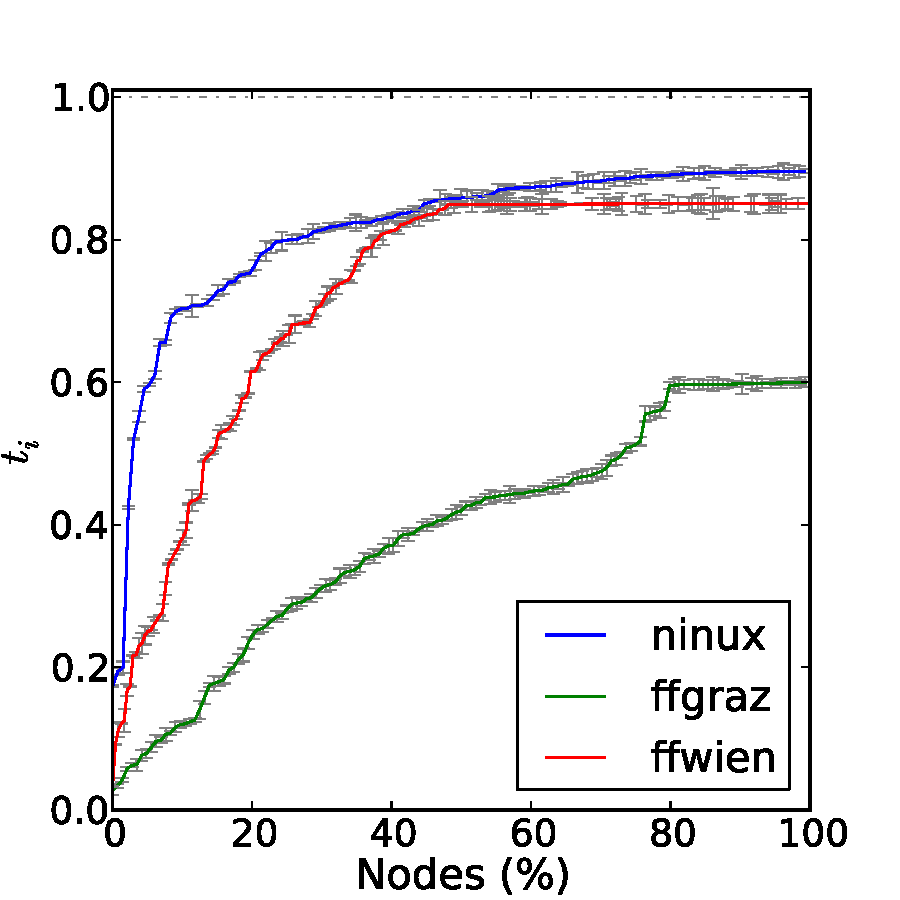
\includegraphics[width=0.49\textwidth]{graphs/all-batman-Tc}
  \hfill
  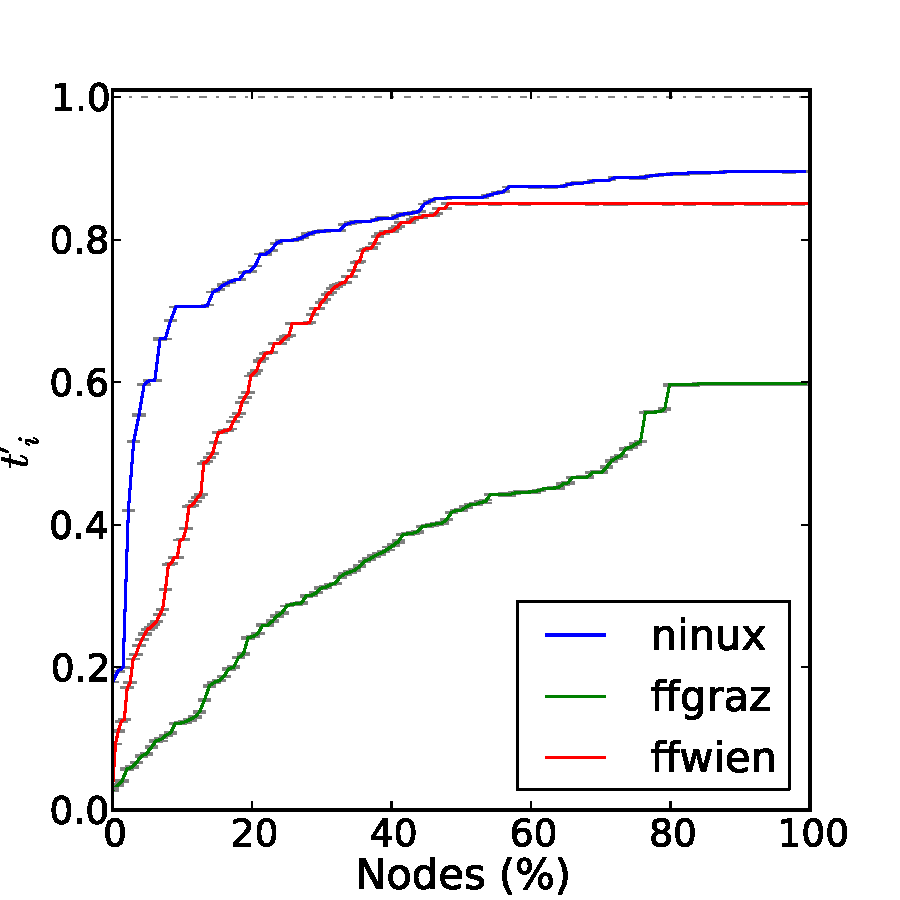
\includegraphics[width=0.49\textwidth]{graphs/all-batman-Rc}
  \hspace*{\fill}
  \caption{Nodes (normalized to 100) ranked by $t_i, t'_i$ in the L-S scenario}
  \label{fig:mp_ls}
\end{figure}

\begin{figure}[htb]
  \centering
  \hspace*{\fill}
  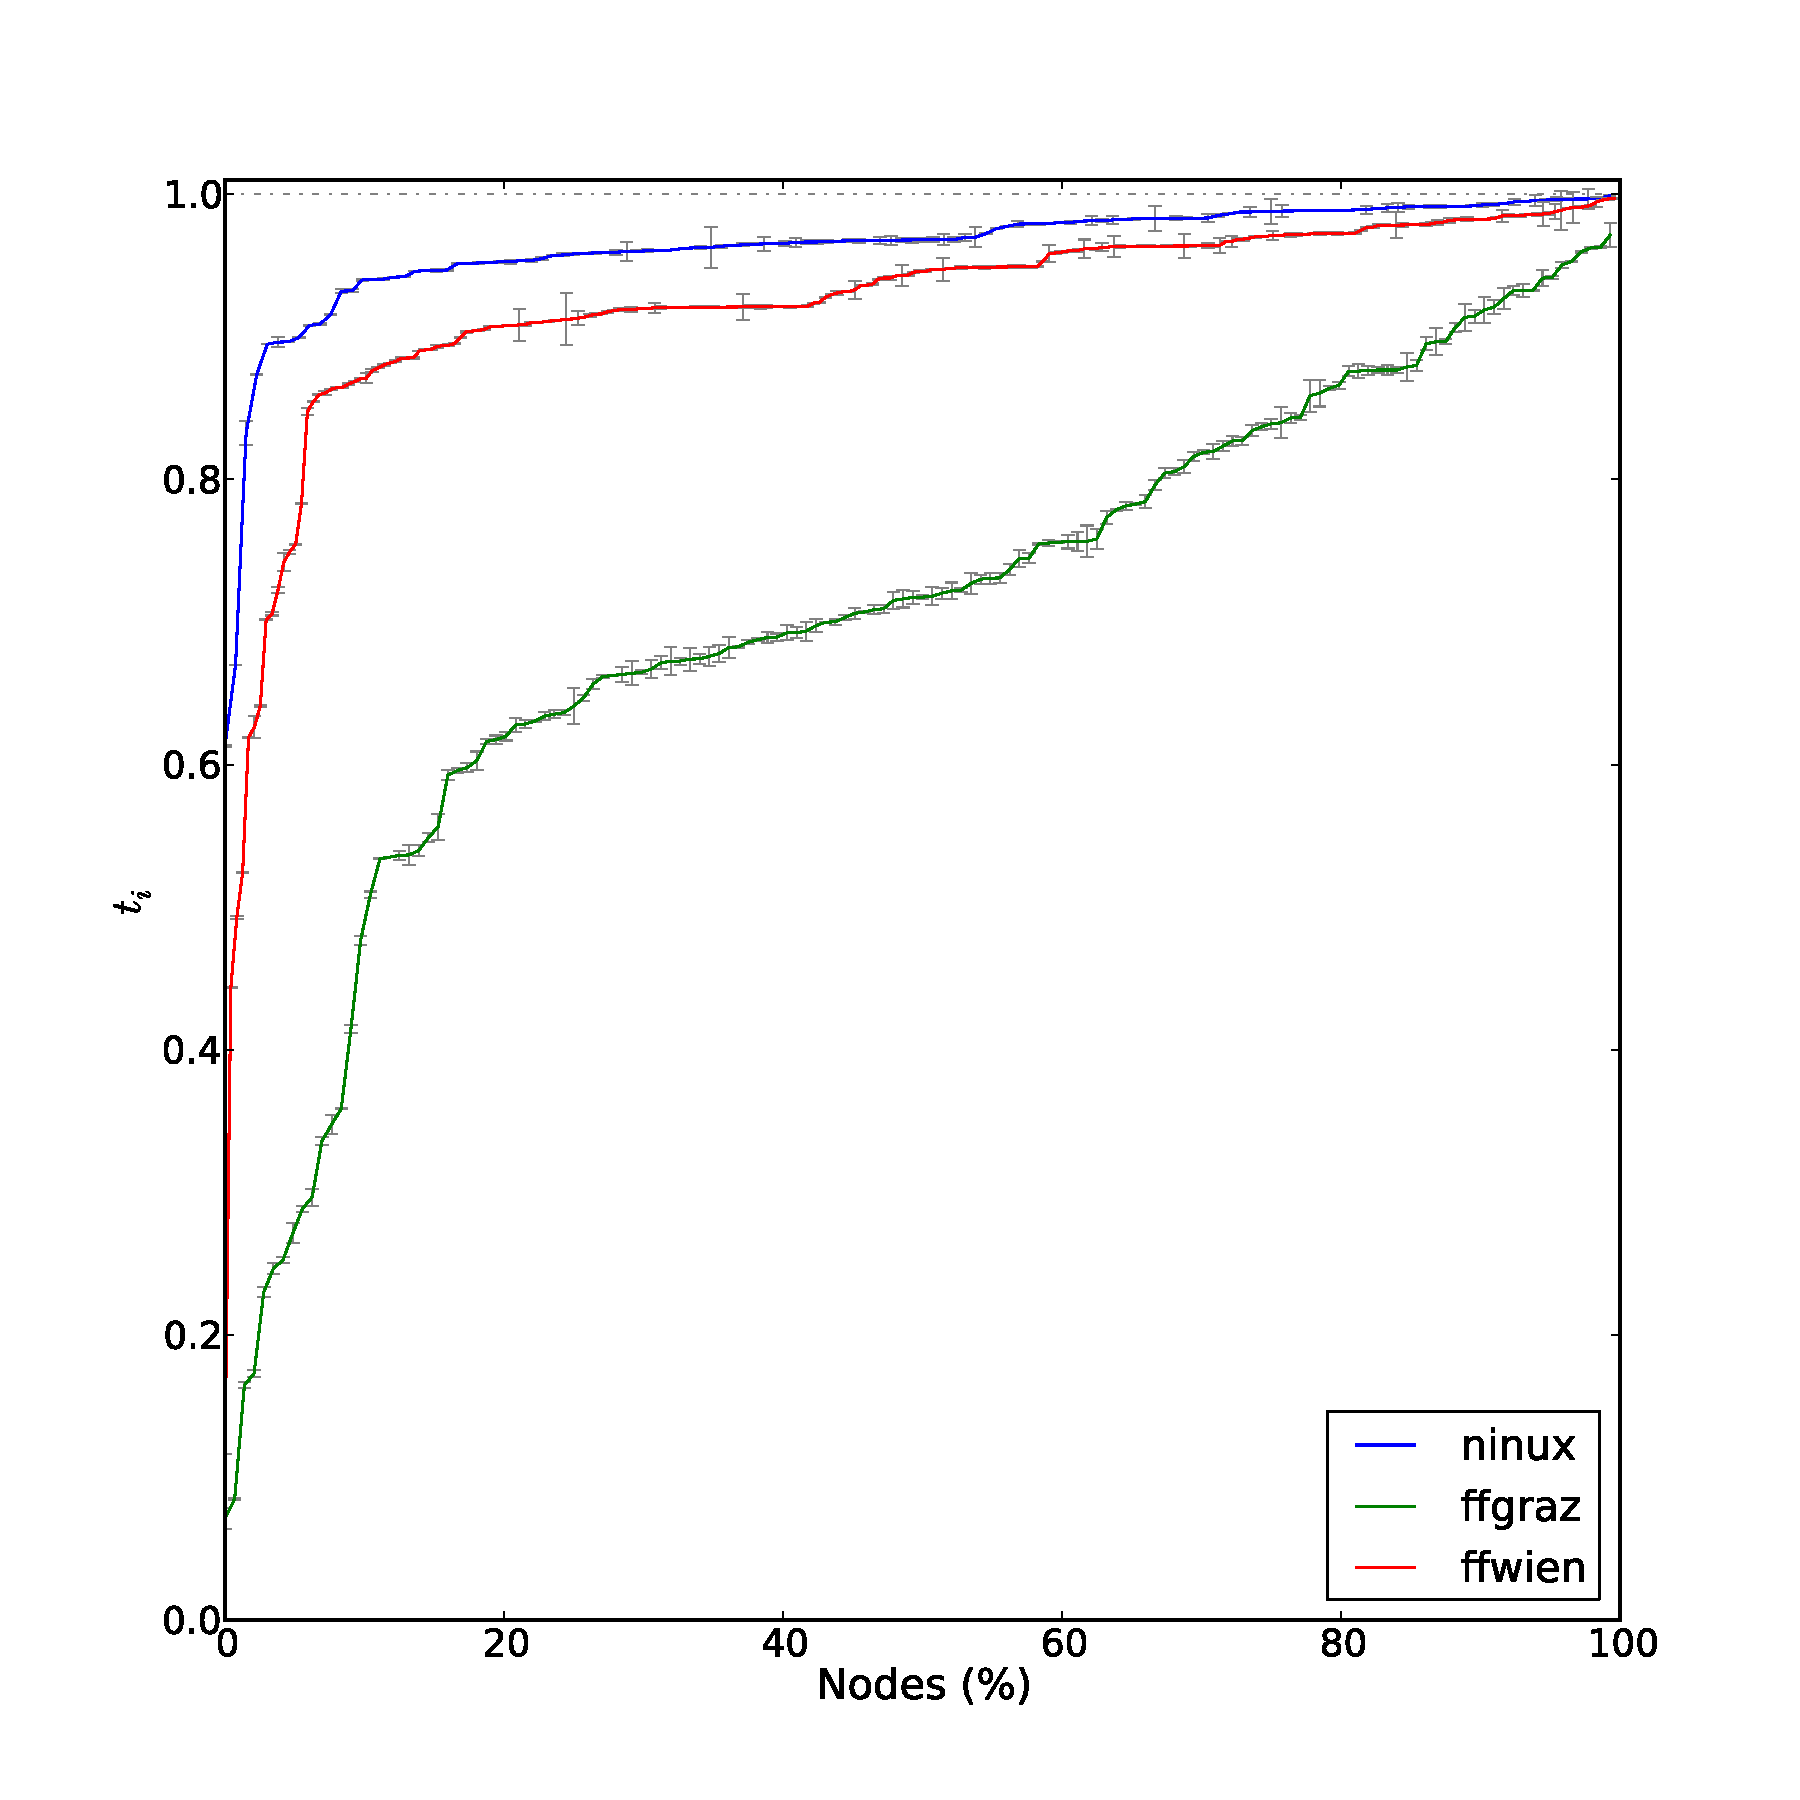
\includegraphics[width=0.49\textwidth]{graphs/all-default-Tc}
  \hfill
  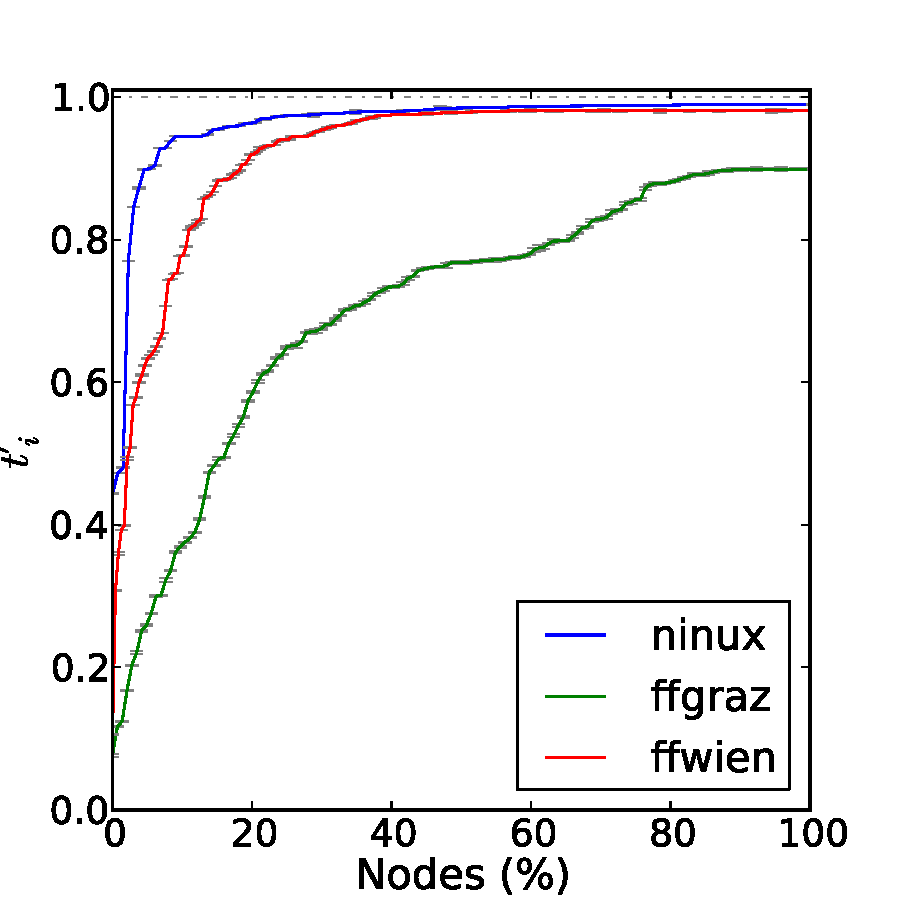
\includegraphics[width=0.49\textwidth]{graphs/all-default-Rc}
  \hspace*{\fill}
  \caption{Nodes (normalized to 100) ranked by $t_i, t'_i$ in the WCN scenario}
  \label{fig:mp_wcn}
\end{figure}

\begin{figure}[htb]
  \centering
  \hspace*{\fill}
  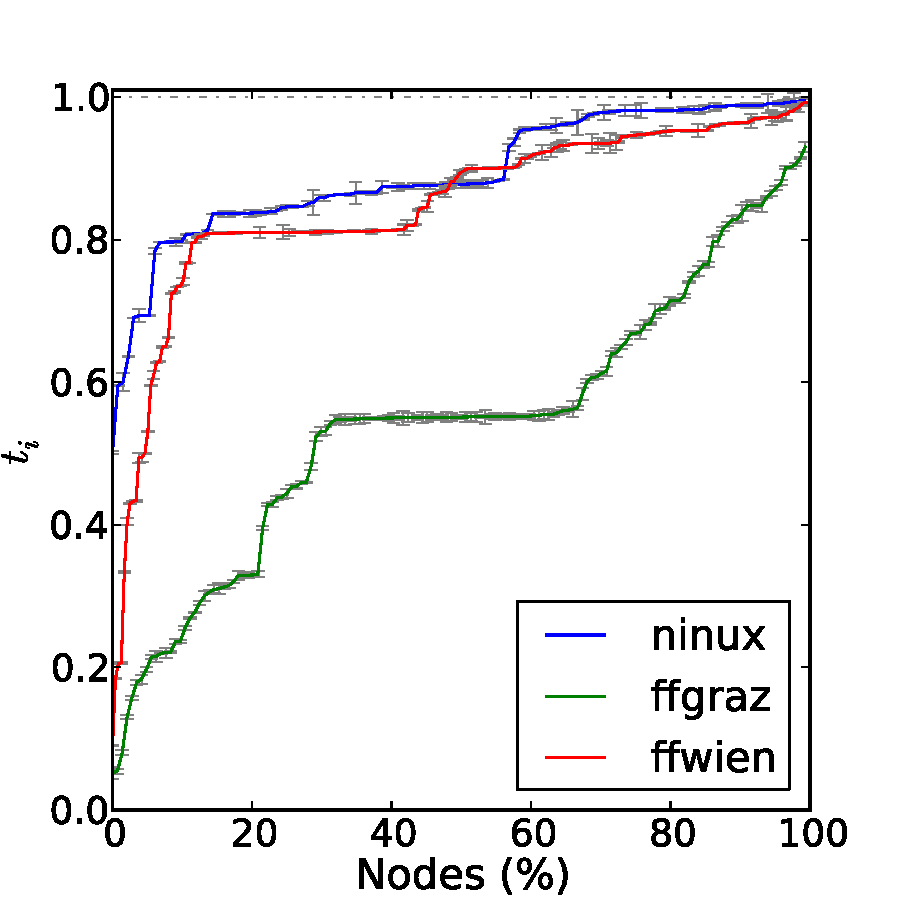
\includegraphics[width=0.49\textwidth]{graphs/all-mpr-Tc}
  \hfill
  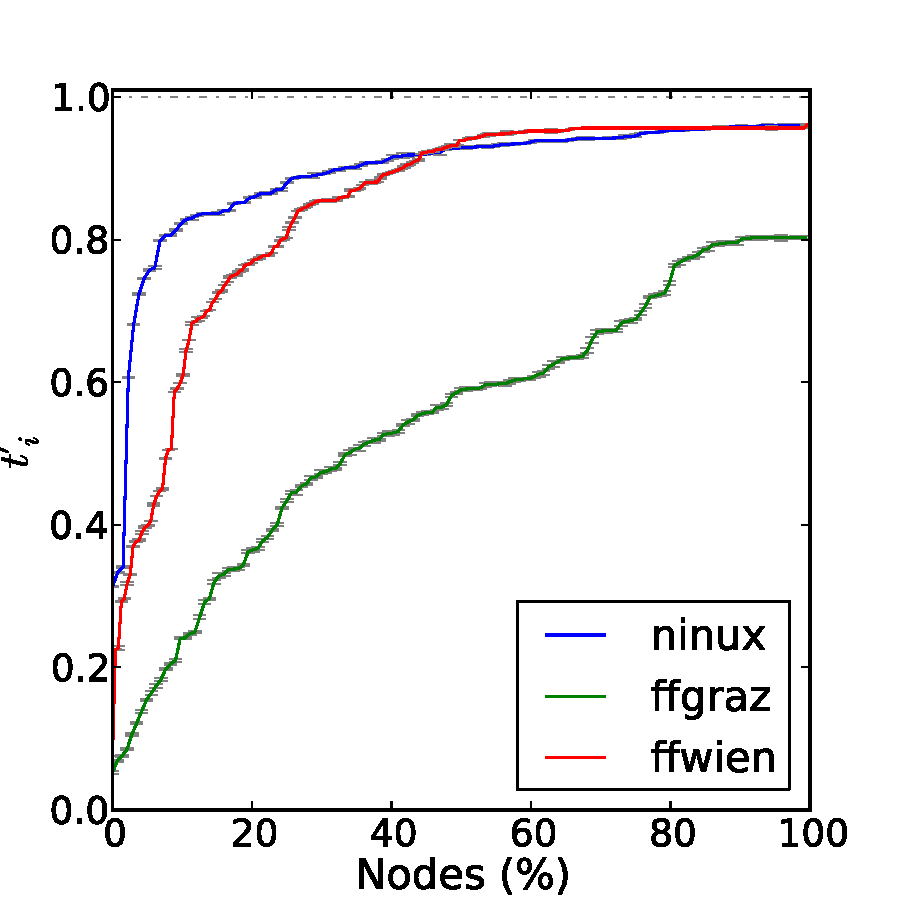
\includegraphics[width=0.49\textwidth]{graphs/all-mpr-Rc}
  \hspace*{\fill}
  \caption{Nodes (normalized to 100) ranked by $t_i, t'_i$ in the OLSR scenario}
  \label{fig:mp_olsr}
\end{figure}

As expected, FunkFeuer Graz is the network that shows the poorest performance,
due to the bad quality of its links and its peculiar topology. Ninux and
FunkFeuer Wien have similar results, with the former responding a bit better.

\figref{fig:mp_ls} shows that nodes have a big difficulty reaching the entire
network with their messages, with no one, even in the best case, exceeding 0.9.
In contrast, \figref{fig:mp_wcn} suggests the importance of transmitting
information about neighbours.

By adding content to the messages, signalling becomes more effective and
less traffic is needed to propagate the required information.
Moreover, in OLSR the discovery of neighbours through \texttt{HELLO}
messages can happen at an higher ratio than the propagation of \texttt{TC}
messages, since they are not flooded.
This introduces a sort of hierarchy: local topology is refreshed more often
in order to propagate more information rich messages to the rest of the network.

A hierarchic approach is precisely what the Open Source implementation of OLSR
uses to ensure that topology information is up to date without suffocating
the network with overhead. The implementers decided to take advantage of the
TTL field in OLSR message and send \texttt{TC} messages with TTL values
different from the default of 255 (the maximum). By sending \texttt{TC}
messages with small (1, 2, 3) TTL values often, the local topology is
updated more frequently without imposing much overhead of the network.
\footnote{\url{http://www.open-mesh.org/projects/open-mesh/wiki/The-olsr-story}}

The addition of MPR forwarding logic (\figref{fig:mp_olsr})
is predictably worse than the WCN scenario,
since redundancy is removed both by the non-use of some links and by some nodes
not generating messages.
Nonetheless, this mode of propagation works substantially better than the L-S
case, for the same reasons described above.

The efficiency of topology information propagation is key to the performance of
a network, at least as much as keeping the routing protocol overhead low.
This analysis considered the propagation of a single message per node, on a
static topology where link costs do not change.
In reality, a link-state protocol is based on the synchronisation of information
between the different nodes. Outdated information may cause routing loops that
completely destroy the throughput.

As a result, it is really important in the design of routing protocols for
wireless mesh networks to account for the need of responding rapidly to
topology changes without overburdening the network in the process.
Some think that proactive link-state protocols may be poor suited in this
situation and research is being carried on to find a better solution.
In the meantime, OLSR is still used, even though not in the way it was designed,
to run some important WCNs with successful results.

\chapter{Conclusions}\label{conclusions}

The first analysis reported in this thesis is the robustness metric.
Different possible real-world scenarios have been simulated, by the usage
of different policies in the removal of nodes and links from the networks.
Random removal was used to simulate independent failures of nodes or links,
while removal of nodes and links with the highest centrality metrics was a
possible interpretation of an attack scenario in which the most important
nodes are maliciously targeted.

The analysis has shown the behaviour of three WCNs and compared it, in the
different analysed scenarios, to the properties of synthetic networks
generated with two random graph models (Erd\H{o}s-Rényi and Bararbási-Albert)
that have a known degree distribution (respectively Poisson and power law).

The fragility of the WCNs has been highlighted, which is partly attributable
to their small density and partly to their peculiar structure. WCN show the
same behaviour in attack scenarios regardless of the centrality metric used
in the simulation. This suggests that, in the three analysed
networks, all the metrics are equivalent in their results.

The Barabási-Albert model, which was expected to give results similar to
those of the WCNs due to its similar degree distribution, had instead shown
some remarkable differences. First of all, in the removal by degree and
betweenness centrality, it remained consistently more robust than the WCNs,
despite a similar density. Secondly, when removing nodes by closeness and
links by betweenness centrality it performed more similarly to the
Erd\H{o}s-Rényi model than to the WCNs.

This findings suggest that the preferential attachment growth model used by
that random graph generator is not really suited for modelling WCNs.
This may be because it does not produce leaves, which are a consistent part
of a WCN; another explanation is that different factors guide the growth of
a WCN, other than the degree of existing nodes.

Subsequently, an analysis of the diffusion of topology information in WCNs
has been performed. Since they use a link-state routing protocol, the correct
propagation of the knowledge about the topology is central in order to avoid
the different nodes having unsynchronised routing tables. Such a situation
may lead to potentially catastrophic effects on the whole network, like the
creation of routing loops.

The two metrics reported by this analysis are: a ranking of nodes by the expected
fraction of other nodes they receive information from; and a ranking by the
expected number of nodes which receive information from them.

The most evident thing that appears by looking at these metrics is that loss
of messages in WCNs is really common on long paths. In WCNs links are highly
heterogeneous, there are really good one as well as really bad ones.
Unfortunately, a single really bad link in a path is enough to jeopardize
all the communications that pass through that path.

Another, more subtle result, obtained by comparing different strategies of
flooding and different kind of link-state advertisement messages, is that
networks benefit from a more frequent diffusion of information on local (nearby)
nodes with respect to information on distant nodes. This produces a beneficial
effect because, with the same frequency of distant node updates, if each nodes
propagates information on its neighbours the distribution is more efficient.

Moreover, since each node can only choose the next hop, the complete and exact
knowledge of the route when doing long distance routing is in most cases
unnecessary and reducing the rate of far reaching topology updates may produce
more advantages than damage.

Some authors, for instance the implementers of the OLSR daemon and of the
B.A.T.M.A.N. routing protocol, suggested that link-state routing protocols,
which presume that each node must have the possibility to calculate every
route, are ill suited to wireless mesh networks, where the topology
is rapidly changing.

Research is ongoing in the field of mesh network routing protocols, and there
is not yet a winner. In the meantime, WCNs all over the world continue
running with a variety of routing protocols and configurations, despite their
weaknesses and shortcomings.
If the situation today appears good for WCNs, it is also clear that there are
large opportunities of technological improvement.

\section{Final remarks}\label{final-remarks}

The software used for the analysis of this thesis has been developed during
my internship with Prof. Renato Antonio Lo Cigno and Dott. Leonardo Maccari
of the ??? laboratory of DISI.

The software, the test cases and the raw result data are available on the public
git repository \dots TODO % TODO

\section{Acknowledgements}\label{acknowledgements}

\chapter*{Bibliography}\label{bibliography}
\addcontentsline{toc}{chapter}{Bibliography}

Barabási, Albert-László, and Réka Albert. 1999. ``Emergence of Scaling
in Random Networks.'' \emph{Science} 286 (5439): 509--12.\\
doi:\href{http://dx.doi.org/10.1126/science.286.5439.509}{10.1126/science.286.5439.509}.
\url{http://www.sciencemag.org/content/286/5439/509}.

Clausen, T., and Philippe Jacquet. 2003. ``Optimized Link State Routing
Protocol (OLSR).'' IETF. \url{http://tools.ietf.org/html/rfc3626}.

De Couto, Douglas {SJ}. 2004. ``High-Throughput Routing for Multi-Hop
Wireless Networks.'' PhD thesis, MIT.
\url{http://citeseerx.ist.psu.edu/viewdoc/download?doi=10.1.1.117.3059\&rep=rep1\&type=pdf}.

Gilbert, E. N. 1959. ``Random Graphs.'' \emph{The Annals of Mathematical
Statistics} 30 (4): 1141--44.
doi:\href{http://dx.doi.org/10.1214/aoms/1177706098}{10.1214/aoms/1177706098}.
\url{http://projecteuclid.org/euclid.aoms/1177706098}.

``List of Wireless Community Networks by Region. Wikipedia, the Free
Encyclopedia.'' 2014. June 10.
\url{https://en.wikipedia.org/w/index.php?title=List_of_wireless_community_networks_by_region\&oldid=612342893}.

Newman, Mark. 2010. \emph{Networks: An Introduction}. Oxford University
Press, USA.

``The history of OLSR'' by the developers of OSLR and B.A.T.M.A.N.
\url{http://www.open-mesh.org/projects/open-mesh/wiki/The-olsr-story}

\end{document}
